\documentclass[extra,mreferee]{gji}
%\usepackage{timet}

\usepackage{graphicx}
\graphicspath{ {./figures} }
\usepackage{subfig}
\usepackage{caption}
\usepackage{floatrow}
\usepackage{amssymb}
\usepackage{commath}
\usepackage{amsmath}
\usepackage[dvipsnames]{xcolor}
\floatsetup[figure]{style=plain,subcapbesideposition=top}
%\usepackage[margin=70mm]{geometry}

%\usepackage{subfig}

\title[Global Adjoint Tomography -- Model GLAD-M25]
  {Global adjoint tomography -- Model GLAD-M25}

\author[Lei et al.]
  {Wenjie Lei$^1$, Youyi Ruan$^{1.2}$, Ebru Bozda\u g$^3$, Daniel Peter$^4$, Matthieu Lefebvre$^1$, \\{\LARGE \rm Dimitri Komatitsch$^5$, Jeroen Tromp$^{1,6}$, Judith Hill$^7$, Norbert Podhorszki$^7$}, \\ {\LARGE \rm and David Pugmire$^7$} \\
  $^1$ Department of Geosciences, Princeton University, Princeton, NJ 08544, USA\\
  $^2$ Nanjing University, Nanjing, China\\
  $^3$ Department of Geophysics, Colorado School of Mines, Colden, CO 80401, USA\\
  $^4$ Extreme Computing Research Center, King Abdullah University of Science and Technology, \\Thuwal 23955-6900, Kingdom of Saudi Arabia\\
  $^5$ LMA, CNRS UPR 7051, Aix-Marseille University, Centrale Marseille, 13453 Marseille Cedex 13, France\\
  $^6$ Program in Applied and Computational Mathematics, Princeton University, Princeton, NJ 08544, USA\\
  $^7$ Oak Ridge National Laboratory, Oak Ridge, TN 37831, USA\\
  }

\newcommand{\btx}{\textsc{BibTeX}}

\begin{document}

\maketitle

\section{Introduction}

{\color{Red} Wenjie: I want to leave this part to the end, when I finished reading all the papers.}

With the development of high performance computing and numerical methods, it is now possible to using adjoint method to image the interior the globe using thousands of earthquakes.

There are few agreements about the earth model and yet many unknown to be resolved. There are quite a lot of global models exits however there is no such con-sense.

The GLAD-M25 is the first earth model that incorporate the P and S wave speed using full waveform inversion. Also, people are using specific set of phases in their inversion. For P models, people are using P phase and other body wave phases and for S models, people are using mostly S wave phases and surface waves to constrain the structure. Those two kinds of models usually reveals very different parts of the earth. For example, for P wave, people used it the image the subduction slabs and it is not very good at image lower mantle structures, such as plumes and lower mantle convection. For S waves, it is the verse verso.

There are many challenges coming along the way. First, the data volume is huge.  There are in total of 1480 earthquakes used in the inversion stage, added into the database step by step. Second, workflow management is crucial dealing with such a large project. One factor is coming from the complex workflow. There are 4 major building blocks, forward simulation, seismic data processing, adjoint simulation and post-processing. Each blocks contains several small blocks. The other factor is coming from the number of earthquakes and high demands of computation. In each iteration, we are doing 1480 forward and adjoint simulation, generating a few Petabytes of wavefield files and consuming 16 million of CPU hours on the supercomputer at Oak Ridge National Lab. There are yet more in data processing stages. How to deal with hardware failures is very important and prevent contamination into our inversion results.

Here, we present our GLAD-M25 earth model, with significantly improvements on the plumes and subductions.

test1 (\cite{zhu2012structure}, \cite{zhu2012structure})
test2 \citep{zhu2015seismic, ekstrom2012global}
test3 \citet{ekstrom2012global}


\section{Starting model GLAD-M15}

As a continuation of our previous work~\citep{bozdaug2016global},
we used ``first generation'' model GLAD-M15 as our
starting model.
GLAD-M15 is a 3D transversely isotropic earth model, which combined
3D mantle model S362ANI~\citep{kustowski2008anisotropic}
with 3D crustal model CRUST2.0~\citep{bassin2000current} as its starting model.
In this study,
we continue to use the same transversely isotropic model parametrization.
Instead of relying on ubiquitous ``crustal corrections'',
the mesh implementation of the crust in the spectral-element solver SPECFEM3D\_GLOBE~\citep{KoTr02a,KoTr02b,PeKoLuMaLeCaLeMaLiBlNiBaTr11} enables us accurately accommodate topography and bathymetry as well as variations in the Moho.
GLAD-M15 was constructed using a global data base of 256 earthquakes.
The first 12 iterations of the GLAD-M15 inversion used three-component seismograms with a shortest period of 27~s,
and the final 3 iterations reduced this further to 17~s.
In this study we also used three-component seismograms with a shortest period of 17~s.

\section{Earthquakes}
\label{section:earthquakes}

\begin{figure}
  \centering
  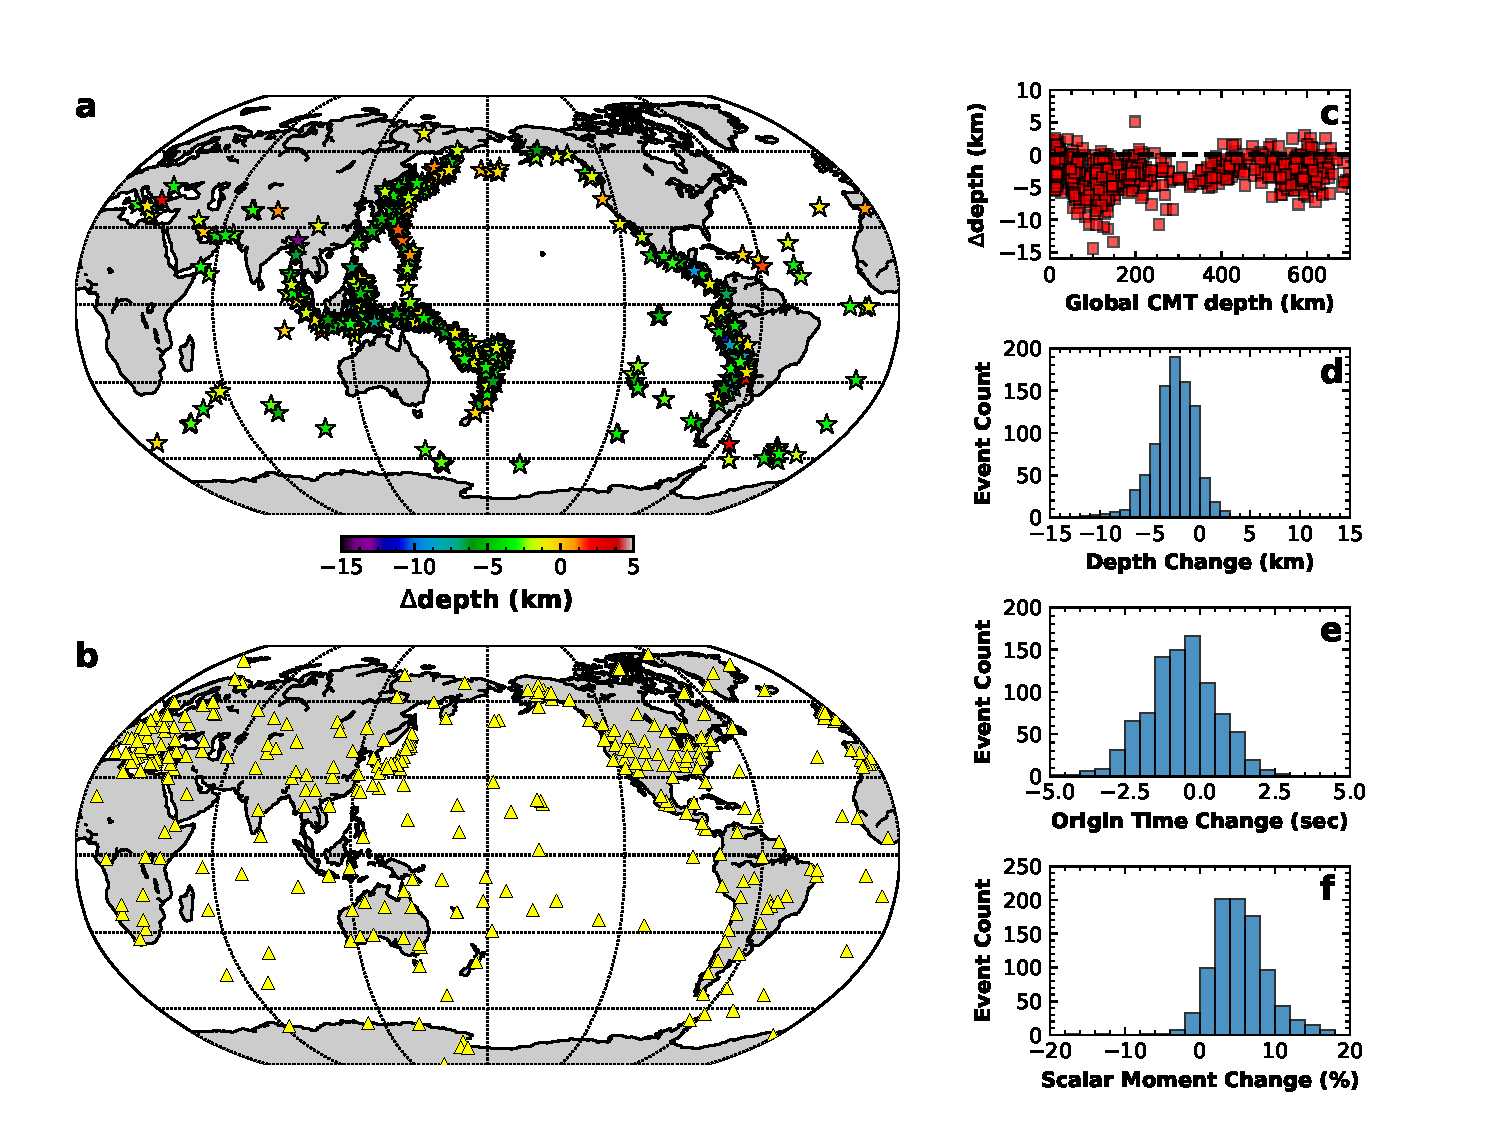
\includegraphics[width=\textwidth]{figures/source_corrections.pdf}
  \caption{Source corrections for 1,040 out of 1,480 events used in the structural inversion. (a) Map view of depth changes. (b) Distribution of seismographic stations used for source inversions. (c) Depth change relative to the original global CMT Catalog depth. (d)--(f) Histograms of depth, origin time, and scalar moment changes relative to the CMT Catalog.
  }
  \label{fig:source_correction}
\end{figure}

In addition to the 256 earthquakes used for the construction of first generation model GLAD-M15, we initially selected 784 carefully chosen additional earthquakes from the global Centroid-Moment Tensor (CMT) catalog~\citep[e.g.,][]{Ekstrom12},
and added them to our database, resulting in a total number of 1,040 earthquakes.
To ensure a good signal-to-noise ratio on a global scale,
the smallest moment magnitude in the database is set to~5.5,
and to avoid complications associated with source size,
the largest moment magnitude is set to~7.2.

Before using the 1,040 earthquakes in our structural inversion,
we performed CMT inversions in model GLAD-M15,
the results of which are summarized in Fig.~\ref{fig:source_correction}.
To ensure even global coverage,
we used seismographic stations from the  Global Seismic Network (II, IU, IC, US, CU, and GT),
GEOFON~(GE), GEOSCOPE~(G), and several regional networks, such as MedNet~(MN),
the Brazilian Lithospheric Seismic Project~(BL), the Chilean National Seismic Network~(C),
and the Japan Meteorological Agency Seismic Network~(JP) (Fig.~\ref{fig:source_correction}b).
The number of stations used for CMT inversion usually ranges
from~150 to~500.

To determine the source parameters in the starting model,
we used the CMT inversion algorithm of \cite{liu2004spectral}.
This algorithm combines a normalized waveform difference misfit with an envelope difference misfit.
Specifically, the algorithm minimizes the misfit function
\begin{equation}
   \begin{split}
      \Phi =  \sum\limits_{c=1}^{C} \omega_c \sum\limits_{r=1}^{R_c} \omega_{cr}
       \sum\limits_{w=1}^{W_{cr}} \omega_{crw}\,
          & \left\{ \lambda\, \frac
              { \int \big[ d_w(t) - s_w(t - \Delta t) \big]^2 \mathrm{d}t}
              {\int \big[ d_w(t) \big]^2  \mathrm{d}t} \right.
       \\ & \quad \left. \mbox{} + (1 - \lambda)\, \frac
              {\int \big[ e(d_w(t)) - e(s_w(t - \Delta t)) \big]^2 \mathrm{d}t}
              {\int \big[ e(d_w(t)) \big]^2\mathrm{d}t} \right\}
              \quad ,
   \end{split}
\end{equation}
where~$d_w(t)$ denotes data in time window~$w$\,,
and~$s_w(t - \Delta t)$ the corresponding synthetic for model~GLAD-M15.
We allow the synthetics to shift relative to the data by an amount~$\Delta t$
--- effectively a station correction --- determined by cross correlation.
The envelope function is denoted by~$e(\,\cdot\,)$\,,
and the parameter~$\lambda$ determines the balance between fitting waveforms versus fitting envelopes.
The number of measurement categories is denoted by~$C$\,.
Following~\cite{ekstrom2012global},
seismograms were filtered between 50~s and 100~s
to select three-component body-wave windows,
and between 60~s and 100~s to select three-component
surface-wave windows,
resulting in six measurement categories, $c=1,\ldots,C$\,.
To balance their contributions,
each category is weighted by the reciprocal of the number of measurements in that
category, $\omega_c$\,.
The number of windows for a given receiver~$r$ in a given measurement category~$c$ is~$W_{cr}$\,.
Each such window is weighted equally, i.e.,~$\omega_{crw}=1$\,.
The number of receivers that records data in category~$c$ is denoted by~$R_c$\,.
As shown in Fig.~\ref{fig:source_correction}b,
the receivers are unevenly distributed across the globe,
with several dense arrays in the Northern Hemisphere and poor coverage in the Southern Hemisphere.
To balance the coverage,
we assign receiver weights~$\omega_{cr}$ based on the expression
\begin{equation}
\omega_{cr}^{-1} = N_c\,\sum_{r'=1}^{R_c} \exp\left[\mbox{}-\left(\frac{\Delta_{rr'}}{\Delta_c}\right)^2\right]
\quad ,
\label{eq:spatial_weights}
\end{equation}
where~$N_c$ is a normalization factor for category~$c$,
and where~$\Delta_{rr'}$ denotes the angular distance between receivers~$r$ and~$r'$\,.
The reference angular distance~$\Delta_c$ for each category~$c$ needs to be chosen such that the condition 
number of the diagonal weighting matrix defined by Eqn.~(\ref{eq:spatial_weights}) is not too large.
The calculation of the weights may be abstracted as: given a spatial distribution of
points on the unit sphere, determine a weighting associated with each point.

The algorithm inverts for the six elements of the moment tensor
and the centroid location~(latitude, longitude, and depth).
The calculation of each associated Fr\'echet derivative requires one full 3D forward simulation,
so, considering we have more than one thousand events,
these source inversions are computationally very expensive.

Because we allow the synthetics to shift by an amount~$\Delta t$ relative to the data,
the CMT inversion has unreliable sensitivity to the centroid time.
To alleviate this problem,
following~\cite{zhu2012structure},
we perform a subsequent grid search for the centroid time and the scalar moment.
The grid-search calibration involves simple shift and multiply operations on seismograms
and, unlike the CMT inversion, requires minimal simulation time.

Most earthquakes show a shallower depth after inversion
(Fig.~\ref{fig:source_correction}c),
consistent with our previous experiences~\citep[e.g.,][]{zhu2015seismic,chen2015multiparameter,bozdaug2016global} and with experiments by~\cite{hjorleifsdottir2010effects}.
We observed an average depth change of~$-2.62\pm2.49$~km relative to the global CMT solutions,
an average scalar moment change of~$5.31\pm3.91$\%,
and an average centroid time shift of~$-0.60\pm1.17$~s.
These are relatively minor corrections, especially in view of the significant expense of the source inversions.
For this reason, when we added another 440 earthquakes during iteration~22,
thereby bringing the total to~1,480 events,
we only performed a grid search to calibrate the centroid times and scalar moments.
Fig.~\ref{fig:event_1480} summarizes the characteristics of all 1,480 earthquakes used in this study.

\begin{figure}
  \centering
  \includegraphics[width=\textwidth]{figures/events_1480.pdf}
  \caption{1,480 earthquakes used in this study. (a) Distribution of earthquakes. The color of each beach ball reflects its depth range, where blue designate events shallower than 50~km, green events between 50~km and 300~km, and red events deeper than 300~km. (b) \& (c) Histograms of earthquake moment magnitudes and depths.}
  \label{fig:event_1480}
\end{figure}


\section{Seismic data}
\label{section:data}

The seismographic stations used in this study were carefully selected to ensure global coverage and high data quality (Fig.~\ref{fig:stations}).
In addition to the seismic stations used for the source inversions,
we included all available data for our 1,480 event earthquake database from many data centers,
including IRIS, ORFEUS, INGV, IPGP, ETH, and GEONET.
Regional and temporary networks,
such as US Array~(TA),
Africa Array~(AF), the Canadian National Seismograph Network~(CN), Geoscience Australia~(AU),
the Antarctic Seismographic Argentinean Italian Network~(AI),
and the New Zealand National Seismograph Network~(NZ),
constitute a significant part
of our database and greatly improve coverage in certain regions.

\begin{figure}
  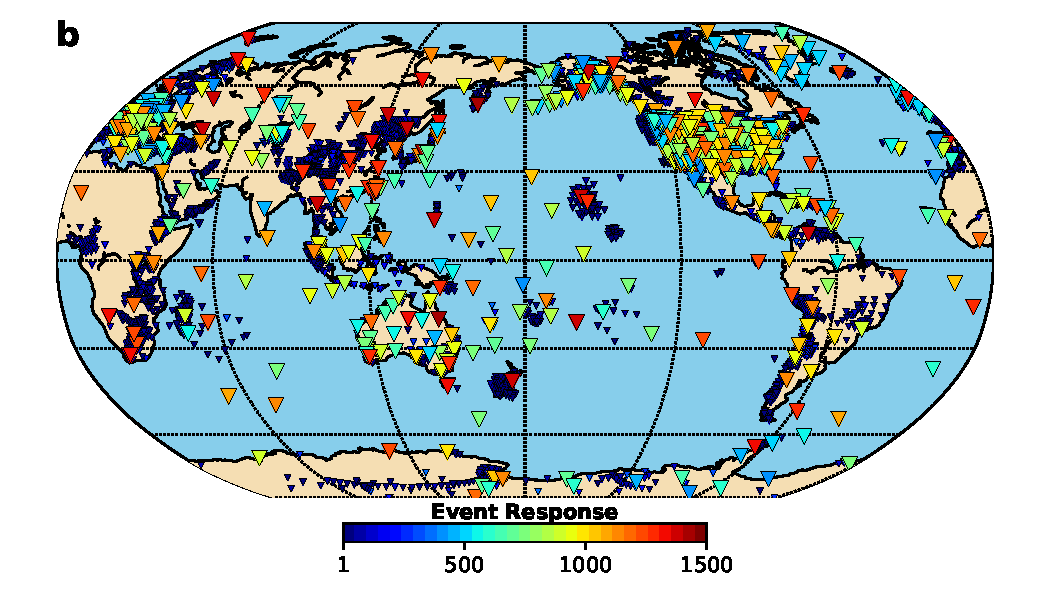
\includegraphics[width=0.8\textwidth]{figures/station_map.pdf}
  \caption{Distribution of 11,800 seismographic stations used in this study. Colors denote the number of events for which a given station contributes waveforms to the structural inversion. Stations with a number of event responses $<400$ are plotted in smaller size; these are usually temporary arrays deployed over a short period of time, frequently ocean bottom seismometers. The maximum number of event responses comes from ANMO, in Albuquerque, New Mexico, which contributed to 1,442 out of 1,480 earthquakes in the data set.}
  \label{fig:stations}
  \centering
\end{figure}

\subsection{Adaptable Seismic Data Format}
\label{section:ASDF}

Conventional seismic data formats, such as SAC, involve one file per time series plus related files with instrument response and event information.
Since every earthquake in the database is typically recorded by thousands of instruments, I/O during the preprocessing stage of the adjoint tomography workflow quickly cripples the file system.
The Adaptable Seismic Data Format (ASDF)~\citep[][ \texttt{https://seismic-data.org/ }]{krischer2016adaptable} was developed with complete reproducibility and fast parallel processing in mind.

In this context, there are four key issues ASDF resolves.
\begin{itemize}
    \item Robustness and stability: the data container is developed and maintained to ensure accuracy of scientific results.
    \item Data organization: the container is self-describing. Data, including waveform, source, and station information, are organized into well-defined structures.
    \item Reproducibility: the container enables scientists to keep track of what has been done to data so that results can be reproduced.
    \item Efficiency: the format provides easy mechanisms for parallel processing.
\end{itemize}
ASDF serves as a self-contained-and-explained data container while taking full advantages of parallel computing.
In our workflow,
one ASDF file contains all the information needed for data processing, including the seismic traces, event information files, and station response files.
The related APIs are carefully designed for easy data extraction and parallel implementation.

\section{Misfit function}
\label{section:misfit}

The misfit function to be minimized during the iterative inversion process must be carefully constructed.
It will typically involve cross-correlation traveltimes for body waves and frequency-dependent multitaper phase measurements for surface waves.
Measurements are made in several passbands of three-component seismograms rotated into vertical, radial, and transverse components, resulting in a number of measurement categories.
In this study, we consider four passbands,
namely, a 17--40~s passband targeting body waves,
two 40--100~s passbands separately targeting body and surface waves,
and a 90--250~s passband targeting longer-period surface waves.
Each passband involves measurements on all three components,
which results in a total of twelve measurement categories.
Although the inversion is designed to minimize the overall misfit,
we will be tracking the misfit reduction in each of the categories to ensure that the model is improving the fit to the data roughly equally across the board.
One of the biggest challenges in the construction of the misfit function is the highly uneven distribution of earthquakes and seismographic stations,
which must be counterbalanced by geographically weighting the data.
This issue is discussed in detail by~\cite{Ruanetal2018};
in this section we present a brief synopsis.

With these considerations in mind,
the overall misfit, $\Phi$, is defined as follows:
\begin{equation}
\label{eq:misfit}
\Phi = \sum_{s}^{S} \omega_s \sum_{c}^{C} \omega_{c} \sum_{r}^{R_{sc}} \omega_{scr} \sum_{w}^{W_{scr}} \omega_{scrw}\, \chi_{scrw}
\quad ,
\end{equation}
where~$S$ denotes the number of sources, $C$ the number of categories,
$R_{sc}$ the number of receivers recording source~$s$ in category~$c$,
and~$W_{scr}$ the number of measurement windows for source~$s$, category~$c$
and receiver~$r$.
The misfit for a specific source~$s$, category~$c$, receiver~$r$, and window~$w$ is
\begin{equation}
  \chi_{scrw} = \frac{1}{\Delta\omega}\int_{\omega_1}^{\omega_2} \Big( \frac {\Delta \tau_{scrw}} {\sigma_{scrw}} \Big)^2\, \mathrm{d}\omega
\quad ,
\end{equation}
where~$\Delta \tau_{scrw}$ denotes a multi-taper frequency-dependent phase measurement over the frequency interval~$\Delta\omega=\omega_2-\omega_1$\,,
with associated standard deviation~$\sigma_{scrw}$\,.
For body waves, the window misfit is simply the cross-correlation traveltime anomaly,
$\Delta T_{scrw}$\,, weighted by its standard deviation, i.e., $\chi_{scrw}=(\Delta T_{scrw}/\sigma_{scrw})^2$\,.
As in the source inversions,
the window weights are equal, $\omega_{scrw}=1$\,,
and the category weight, $\omega_c$\,, is the reciprocal of the number of measurements in that
category.
Earthquakes are mainly confined to plate boundaries,
and most seismic stations are confined to the continents,
which leads to a very uneven distribution of sources and stations,
as illustrated in Figs.~\ref{fig:event_1480} and~\ref{fig:stations}.
Therefore, weighting is crucial in global tomography to balance this uneven sampling
of Earth's interior.
Our source and receiver weighting strategy,
encapsulated by the weights~$\omega_s$ and $\omega_{scr}$\,,
is developed to compensate for uneven spatial sampling.
Following the same strategy as for the receiver weights in the source inversions,
we define the source and receiver weights as
\begin{equation}
\omega_{s}^{-1} = N\,\sum_{s'=1}^{S} \exp\left[\mbox{}-\left(\frac{\Delta_{ss'}}{\Delta}\right)^2\right]
\quad ,
\label{eq:source_weights}
\end{equation}
and
\begin{equation}
\omega_{scr}^{-1} = N_{sc}\,\sum_{r'=1}^{R_{sc}} \exp\left[\mbox{}-\left(\frac{\Delta_{rr'}}{\Delta_{sc}}\right)^2\right]
\quad ,
\label{eq:receiver_weights}
\end{equation}
respectively.
Here~$N$ and~$N_{sc}$ are a normalization factors,
and~$\Delta_{ss'}$ and~$\Delta_{rr'}$ denote angular distances between source and receiver pairs~$\{s,s'\}$ and~$\{r,r'\}$\,.
The reference angular distances~$\Delta$ and~$\Delta_{sc}$ need to be chosen based on the condition 
numbers of the diagonal weighting matrices defined by Eqns.~(\ref{eq:source_weights}) and~(\ref{eq:receiver_weights}).

\section{Model parametrization}

We use the same transversely isotropic model parametrization as starting model GLAD-M15.
Such a model is described by the five Love parameters $A$, $C$, $L$, $N$, and $F$~\citep{Love27},
or, alternatively, using the mass density~$\rho$, in terms of the wavespeeds~$\alpha_v=\sqrt{C/\rho}$, $\alpha_h=\sqrt{A/\rho}$, $\beta_v=\sqrt{L/\rho}$, $\beta_h=\sqrt{N/\rho}$ and the dimensionless parameter $\eta=F/(A-2L)$~\citep{PREM,DT98}.
Assuming the radial anisotropy is due to shear anisotropy, these five parameters
may be further reduced to four by introducing the bulk sound speed,
$c=\sqrt{\kappa/\rho}$\,.
Therefore, the final four parameters are $c$, $\beta_v$, $\beta_h$, and $\eta$.

Since density is difficult to constrain with seismic data,
density perturbations are scaled to isotropic (Voigt averaged) shear wavespeed perturbations based on the relationship~$\delta\ln\rho = 0.33\,\delta\ln\beta$~\citep{montagner1989petrological}.

Based on this parametrization,
the variation in the misfit function~(\ref{eq:misfit}) may be expressed as~\citep{zhu2015seismic,bozdaug2016global}
\begin{equation}
    \delta \Phi = \int_V
      (\delta \ln c\,K_c + \delta \ln\beta_v\,K_{\beta_v} + \delta \ln\beta_h\,K_{\beta_h} +
      \delta\ln\eta\,K_\eta) \mathrm{d}V
      \quad ,
\end{equation}
where~$K_c$, $K_{\beta_v}$, $K_{\beta_h}$, and $K_\eta$ denote the four Fr\'echet derivatives,
which are calculated based on an adjoint-state method~\citep[e.g.,][]{Plessix_2006_RAS,Tromp2005}.

\section{Adjoint tomography workflow}

The adjoint tomography workflow is shown in Fig.~\ref{fig:adjoint_workflow}.
It starts with the selection of earthquakes, as discussed in Section~\ref{section:earthquakes}.
Given the earthquake selection,
observed seismographic data and related response information are acquired,
as discussed in Section~\ref{section:data}.
For a given earthquake,
the corresponding seismograms and related response information are combined in a single ASDF file,
described in Section~\ref{section:ASDF}.
For a given earthquake dataset, the conversion to ASDF needs to be performed once and for all.
In the following sections we highlight several important aspects of the workflow.

\begin{figure}
  \centering
  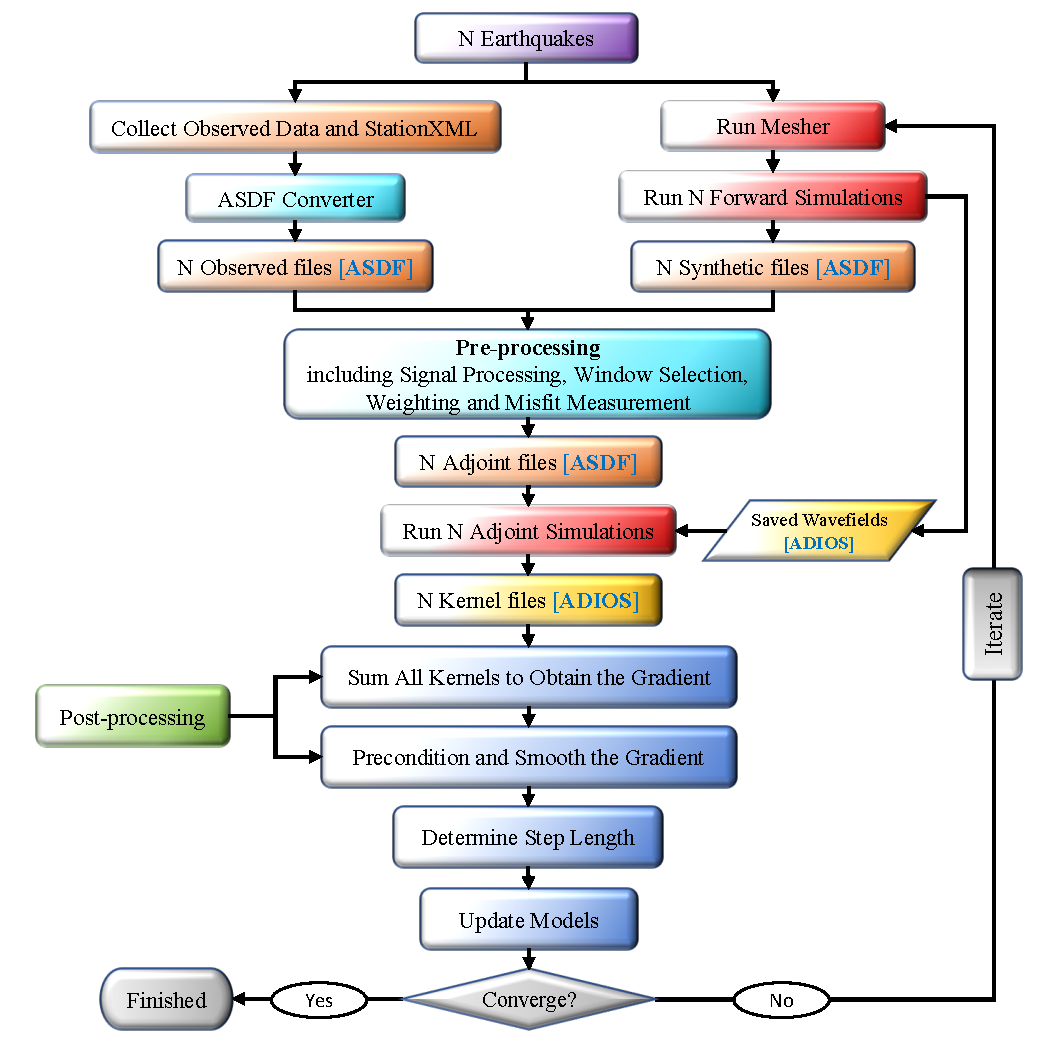
\includegraphics[width=\textwidth]{figures/adjoint_workflow_6.pdf}
  \caption{Adjoint tomography workflow.}
  \label{fig:adjoint_workflow}
\end{figure}

\subsection{Forward simulations}

The observed seismograms need to be compared to corresponding synthetic seismograms
for the purpose of making measurements.
The forward simulations are based on the global spectral-element solver SPECFEM3D\_GLOBE~\citep{KoTr02a,KoTr02a},
and take a CMT solution, a relevant list of stations, and the current earth model as input.
The solver is GPU accelerated, and the simulations are performed on the Cray `Titan' at the Oak Ridge Leadership Computing Facility.
To simulate 120~min seismograms with a shortest period of 17~s on 384 NVIDIA Tesla K20X GPUs takes approximately 10~min of wall clock time.
The calculation of Fr\'echet derivatives at a later stage of the workflow requires access to snapshots of the forward wavefield as part of the parsimonious storage algorithm developed by~\cite{KoXiBoPeSaLiTr16},
with rapid I/O facilitated by ADIOS~\citep{liu2014hello}.
For the current simulation setup,
this requires about 1~TB of storage per earthquake,
so for 1,480 earthquakes this amounts to 1.5~PB of storage.

\subsection{Seismic data processing}

\begin{figure}
  \centering
  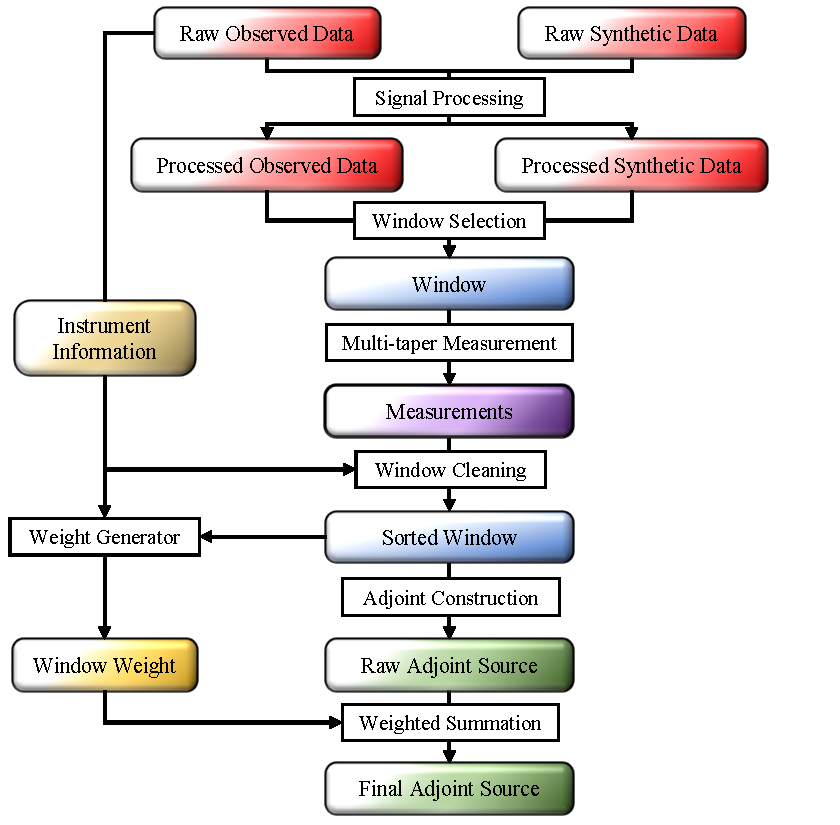
\includegraphics[width=0.8\textwidth]{figures/Preprocess_workflow.pdf}
  \caption{Preprocessing workflow for seismic data.}
  \label{fig:preprocess_workflow}
\end{figure}

The seismic data preprocessing workflow takes raw observed and synthetic data as input,
and generates adjoint sources for data assimilation as output.
From a computational perspective, the preprocessing workflow consumes only~1\% of the overall computational requirements.
But from the perspective of the tomographic inversion, this is by far the most important stage of the adjoint tomography workflow,
directly and fundamentally impacting the outcome.
Any ``bad data'' assimilated at this stage may contaminate the gradient and ultimately the final model.

We use millions of seismograms generating tens of millions of measurement windows,
making data selection through human interaction impossible.
The preprocessing workflow automates this task,
most importantly via the time window selection tool FLEXWIN~\citep{maggi2009automated}.
Every seismogram and potential measurement goes through multiple checks and and balances before acceptance or rejection.

As illustrated in Fig.~\ref{fig:preprocess_workflow}, the preprocessing workflow includes the following phases.
\begin{enumerate}
  \item Signal processing to remove the instrument response from observed data
    to recover ground displacement. Both observed and synthetic data are bandpass
    filtered, and the horizontal components are rotated to obtain the radial and transverse components of motion.
  \item Window selection on a pair of
    observed and synthetic seismograms. Pyflex (a Python version
    of FLEXWIN) is
    used to automatically generate windows where observed and
    synthetic data are sufficiently close to make measurements based on user defined
    criteria.
  \item Cross-correlation traveltime or multi-taper phase measurements in selected windows.
  \item Window sorting and cleaning based on statistical analyses of all measurements to eliminate outliers.
  \item Preliminary adjoint source construction based on the sorted windows.
  \item Calculation and assignment of weights, as discussed in Section~\ref{section:misfit}.
  \item Construction of the final, properly weighted, adjoint sources.
\end{enumerate}

\subsection{Adjoint Simulations}

Collectively,
the adjoint simulations are the most expensive stage of the adjoint tomography workflow. 
Adjoint simulations take the adjoint sources as input, and generate Fr\'echet
derivatives of the four model parameters as output.
The computational cost of one adjoint simulation is roughly twice ($\sim25$~min) that of a forward simulation,
since the forward wavefield is recalculated for convolution with the adjoint wavefield during the adjoint simulation,
as discussed in~\cite{KoXiBoPeSaLiTr16}.
Using this procedure,
both the forward and adjoint wavefield are calculated in forward time,
and attenuation is accurately taken into account in both simulations.

\subsection{Postprocessing}

The postprocessing stage of the workflow takes Fr\'echet derivatives as input and
generates a model update as output.
It involves the follow steps.
\begin{enumerate}
  \item Summation of the individual Fr\'echet derivatives for each earthquake to obtain the overall gradient of the misfit function. The contribution of each source is weighted to balance
    the uneven distribution of earthquakes based on the weighting strategy discussed in Section~\ref{section:misfit} .
  \item Smoothing of the raw misfit gradient using a 3D Gaussian, which
    serves as a regularization procedure. Instead of using a changing
    smoothing radius based upon the ``ray density''~\citep{bozdaug2016global},
    we used a fixed value at a given iteration, following~\cite{zhu2012structure}.
  \item Preconditioning of the smoothed gradient based on a technique proposed by~\cite{luo2013strategies}.
  \item Line search to determine the magnitude of the model update.
  The search direction is determined using a nonlinear conjugate gradient method~\citep{wright1999numerical} (iterations 16--21) or an L-BFGS quasi-Newton method (iterations 22--25).
  We used a subset of 120 earthquakes to conduct the line search and determine the step length.
\end{enumerate}

\subsection{Workflow management}

There are more than ten stages in the adjoint tomography workflow,
and each stage involves thousands of small tasks.
For every model iteration,
we perform 1,480 forward and adjoint simulations, each involving hundreds of compute cores and graphics cards, as well as heavy I/O.
The workflow is prone to human error and hardware failure, making it fragile.
For these reasons, we wish to harden the worflow by taking advantage of modern workflow management software.
With this goal in mind, we selected RADICAL-SAGA and RADICAL-EnTK as our workflow management engines, and developed complementary seismic tomography workflow tools~\citep{EnTK2017}.
The workflow engine can automatically detected job failures both from the HPC system and via user-defined functions.
This enables us to keep track of all tasks and semi-automatically resubmit jobs if necessary.
Given that most HPC system time is spent waiting in the job queue, automatic failure detection and relaunching greatly shortens the overall time to solution.

\section{Misfit evolution}

The inversion went through ten iterations in a number of stages, as documented in this section.
The evolution of the overall misfit function~(\ref{eq:misfit}) as well as its behavior in the various measurement categories is summarized in Fig.~\ref{fig:misfit}.

\begin{figure}
  \centering
  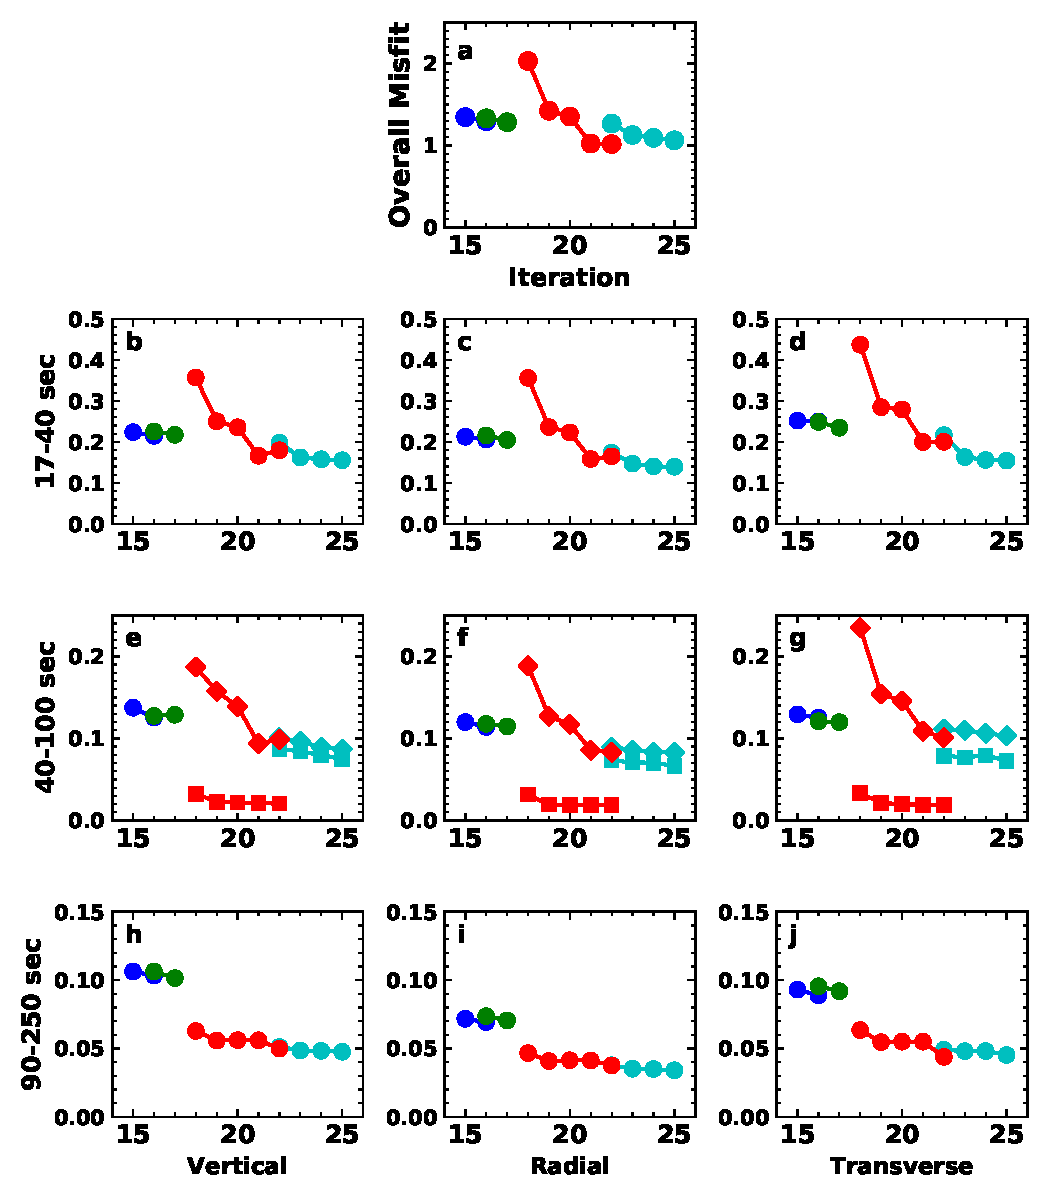
\includegraphics[width=0.8\textwidth]{figures/misfit.pdf}
  \caption{Evolution of phase misfits from GLAD-M15 to GLAD-M25.
  Each color denotes the different stages of inversions, between
  which we make changes to the inversion by either tuning the
  weighting strategies or adding more data.
  (a) Evolution of the total phase misfit. (b) - (j) Misfit in
  each period band and component. (e) - (g) From GLAD-M18,
  we future split the 40-100 sec period band into two
  measurement categories: body(red diamond) waves and surface waves
  (red square).
  {\color{red} Wenjie, why do the graphs overlap at iteration 22, but not at iteration 18? Shouldn't 22 look like 18, i.e., no overlapping points?    \textbf{To Jeroen}: overlap means I calculate the misfit twice using the same mode. For example, in iteration M22, I caculated the misfit using the 1040 earthquakes and 1480 earthquakes, respectively. In M18, I haven't done so. If you want, I can calculate the misfit values and adding the overlap misfit point.}
  {\color{blue}Wenjie: OK, then let's be consistent in what we do. I would prefer no overlap.}
  }
  \label{fig:misfit}
\end{figure}

\subsubsection{Stage~I: Iterations 15--17}

Starting model GLAD-M15 was constructed using a database of 256 earthquakes.
For iterations 15--17 of the inversion we used an expanded database of 520 events.
Our focus was to validate and test our software and workflow before scaling up
to a larger database of 1,040 events.
For these iterations we used three period bands, namely,
17--40~s, 40--100~s, and 90--250~s,
and we used a nonlinear conjugate
gradient method to update the model.

\subsubsection{Stage~II: Iterations 18--21}

We see an abrupt change in the value of the misfit function at iteration 18
in Fig.~\ref{fig:misfit},
reflecting the addition of 520 events to the inversion database,
and a change in the weighting strategy for 40--100~s surface waves.
For iterations 18--21 we split the 40--100~s period band into two, separating the body and surface waves (Figs.~\ref{fig:misfit}e--g).
Since body and surface waves sample different parts of the mantle,
this split facilitated more control over the spatial distribution of the model update.
Because the 17th iteration model explains 40--100~s surface wave data relatively well,
we reduced their weight on all three components for iterations 18--21,
as indicated by the lower red curves in Figs.~\ref{fig:misfit}e--g.

The misfit reduction for 17--40~s body waves (Figs.~\ref{fig:misfit}b--d) tapers off by iteration 21, prompting us to add more earthquakes and change the weighting strategy again by reintroducing the 17--40~s surface waves.

% Table~\ref{table:measurement_category} shows the four passbands we used in Stage~II, tabulating misfit reductions in all four passbands on three components,
% that is, in twelve measurement categories.

% \begin{table}[!htb]
%   \centering
%   \begin{tabular}{|c|c|c|c|}
%     \hline
%     ~          &  Vertical & Radial &  Transverse \\
%     \hline
%     17--40~s   &   P-SV          & P-SV           & SH   \\
%     40--100~s  &   P-SV          & P-SV            & SH \\
%     40--100~s  &   Rayleigh   & Rayleigh    & Love \\
%     90--250~s  &   All                 & All                  & All  \\
%     \hline
%   \end{tabular}\\
%   \caption{Twelve measurement categories used for iterations 18--25.
%   Before iteration~18, the 40--100~s body and surface waves categories were combined into a single category on each component, resulting in nine categories.}
%   \label{table:measurement_category}
% \end{table}

\subsubsection{Stage~III: Iterations 22--25}

At iteration~22 we added another 440 earthquakes to the database,
bringing the total to 1,480 event,
and we changed the 40--100~s surface wave weights back to their setting in Stage~I.
During this stage we switched from a nonlinear conjugate gradient optimization algorithm to an L-BFGS quasi-Newton method.

\subsection{Misfit assessment}
\label{section:Misfit assessment}

In the previous sections we discussed the evolution of the misfit through three key stages of the inversion.
It is important to note that ``the misfit function'' is, in fact, a continually moving target, because at every iteration the number of measurements increases as the model improves,
and the number of earthquakes increases at iterations~18 and~22.

In this section we calculate specific changes in misfit using all 1,480 earthquakes and an identical set of weightings and windows for three models, namely, GLAD-M25, GLAD-M15, and S362ANI combined with CRUST2.0.
Table~\ref{table:misfit_reduction_M15_M25} summarizes the changes in fit in the twelve measurement categories
between the new model, GLAD-M25, and its starting model, GLAD-M15, and between GLAD-M25 and model S362ANI combined with CRUST2.0, which was the starting model for the GLAD-M15 inversion.
In all categories we observe significant misfit reductions,
with dispersive 40--100~s surface waves exhibiting the largest improvements.
The improvements in fit per component are comparable in all period bands,
indicating that the various categories are reasonably well balanced in the assessment of misfit.

%{\color{red} Wenjie: Make sure the variance reductions are calculated as ln (Phi\_M25 / Phi\_M15).}
%{\color{red} Wenjie: I was using (Phi\_M25 - Phi\_M15) / Phi\_M15. So let me modify it?}
%{\color{blue} Wenjie: yes please. It will only change things slightly, if at all. You need to do the same for Table~\ref{table:misfit_reduction_M15_M25_360}.}

\begin{table}[!htb]
  \centering
  \begin{tabular}{|c|c|c|c|}
    \hline
    ~          &  Vertical (\%) & Radial (\%) &  Transverse (\%) \\
    \hline
    %17--40~s  body waves    &   17.4 (31.1)   &       21.1 (37.1) &       24.6 (42.2) \\
    %40--100~s body waves    &   16.8 (31.3)  &       21.3 (40.2)  &       21.7 (42.0) \\
    %40--100~s surface waves &   28.5 (50.1)  &       28.3 (51.1) &       28.4 (53.8)  \\
    %90--250~s surface waves &   14.5 (36.2)  &       13.4 (38.8) &       25.7 (38.6) \\
    17--40~s  body waves    &   19.1 (37.3)   &       23.7 (46.3) &       28.2 (54.8) \\
    40--100~s body waves    &   18.3 (37.5)   &       24.0 (51.4) &       24.5 (54.5) \\
    40--100~s surface waves &   33.6 (69.6)   &       33.3 (71.5) &       33.5 (77.2) \\
    90--250~s all waves &   15.7 (44.9)   &       14.4 (49.1) &       29.6 (48.7) \\
    \hline
  \end{tabular}\\
  \caption{Changes in fit in the twelve measurement categories
  between the new model, GLAD-M25, and its starting model, GLAD-M15,
  and, in parentheses, between GLAD-M25 and model S362ANI combined with
  CRUST2.0, which was the starting model for the GLAD-M15 inversion.}
  \label{table:misfit_reduction_M15_M25}
\end{table}

% \begin{table}[!htb]
%   \centering
%   \begin{tabular}{|c|c|c|c|}
%     \hline
%      ~          &  Vertical(\%) & Radial(\%) &  Transverse(\%) \\
%     \hline
%     17--40s body waves     &    31.1    &       37.1 &       42.2 \\
%     40--100s body waves    &    31.3    &       40.2 &       42.0 \\
%     40--100s surface waves &    50.1    &       51.1 &       53.8 \\
%     90--250s               &    36.2    &       38.8 &       38.6 \\
%     \hline
%   \end{tabular}\\
%   \caption{Misfit Reduction from M00 to M25 for 1480 earthquakes used in the inversion}
%   \label{table:misfit_reduction_M00_M25}
% \end{table}

\subsection{Histogram comparisons}
\label{section:Histogram comparisons}

Another way to evaluate model performance is by assessing the distribution
of measurements in the various categories.
Again we use all 1,480 events and a set of identical windows on all three components
to assess GLAD-M25, GLAD-M15, and S362ANI combined with CRUST2.0.
The total number of selected windows exceeds 18~million.
Fig~\ref{fig:phase_hist} shows histograms of the resulting phase
measurements in all twelve measurement categories.
We observe that the distributions generally become better centered on zero,
and that all standard deviations are steadily reduced.
Again we note that the inversion is aimed at reducing the overall misfit,
so there are small tradeoffs between different measurement categories.

Fig~\ref{fig:amp_hist} shows histograms of the amplitude
measurements for all twelve measurement categories,
which were not used in the current inversion.
Despite this,
we observe modest reductions in all standard deviations of the histograms.
The histograms are nicely centered, indicating that the moment magnitudes are suitably selected, because the scalar moment affects all measurement categories equally.
In the next phase of our ongoing inversion we plan to begin assimilating amplitude measurements,
while simultaneously adding shear attenuation as a new model parameter.

\begin{figure}
  \centering
  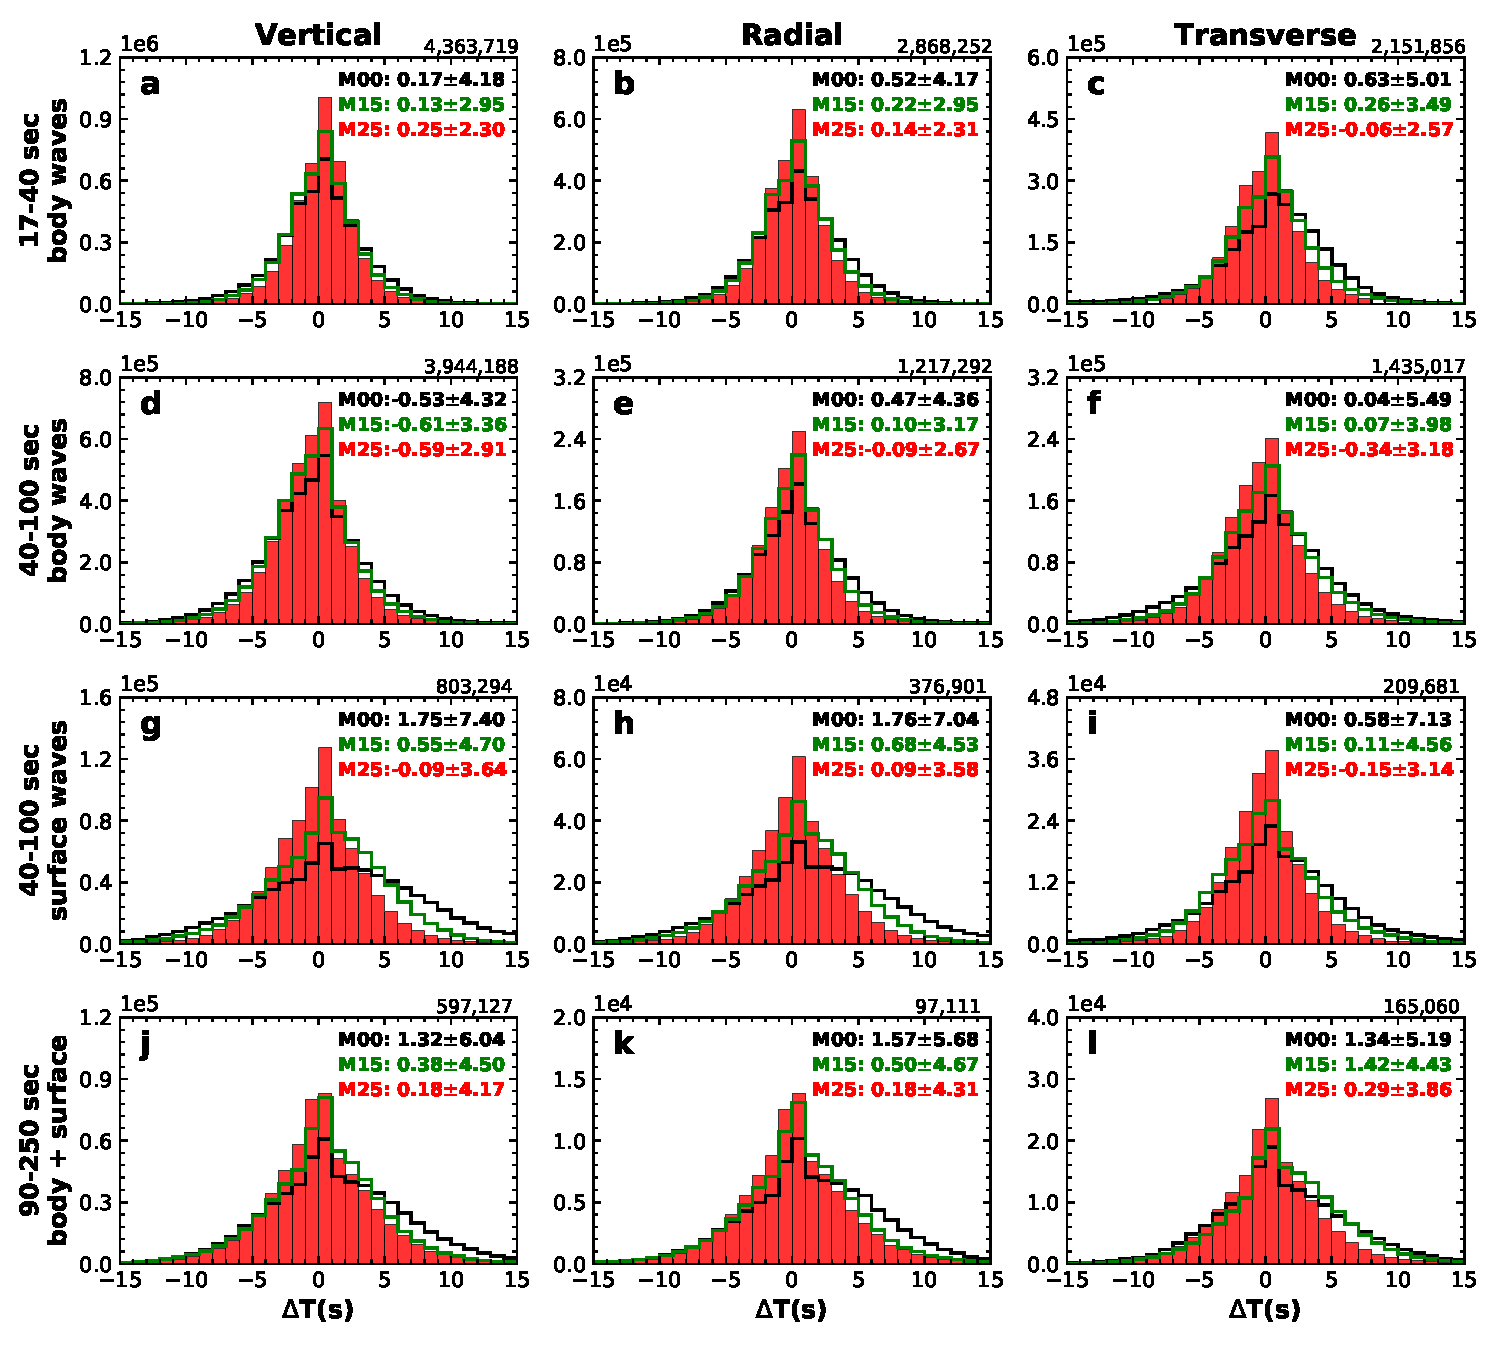
\includegraphics[width=\textwidth]{figures/dt_histogram.pdf}
  \caption{Histograms of phase measurements in all twelve measurement categories for S362ANI combined with CRUST2.0 (M00, \textbf{Black}), GLAD-M15 (M15, \textbf{{\color{ForestGreen} Green}}) and GLAD-M25 (M25, \textbf{{\color{Red} Red}}).
  Each column represents one component, and each row corresponds to a period band.
  The numbers above the top right of each panel denote the number of measurements in the corresponding category.
  The total number of measurements is 18.2 million.
  The mean and standard deviations of the phase measurements for the three models are displayed in the top right corner of each panel.}
  \label{fig:phase_hist}
\end{figure}

\begin{figure}
  \centering
  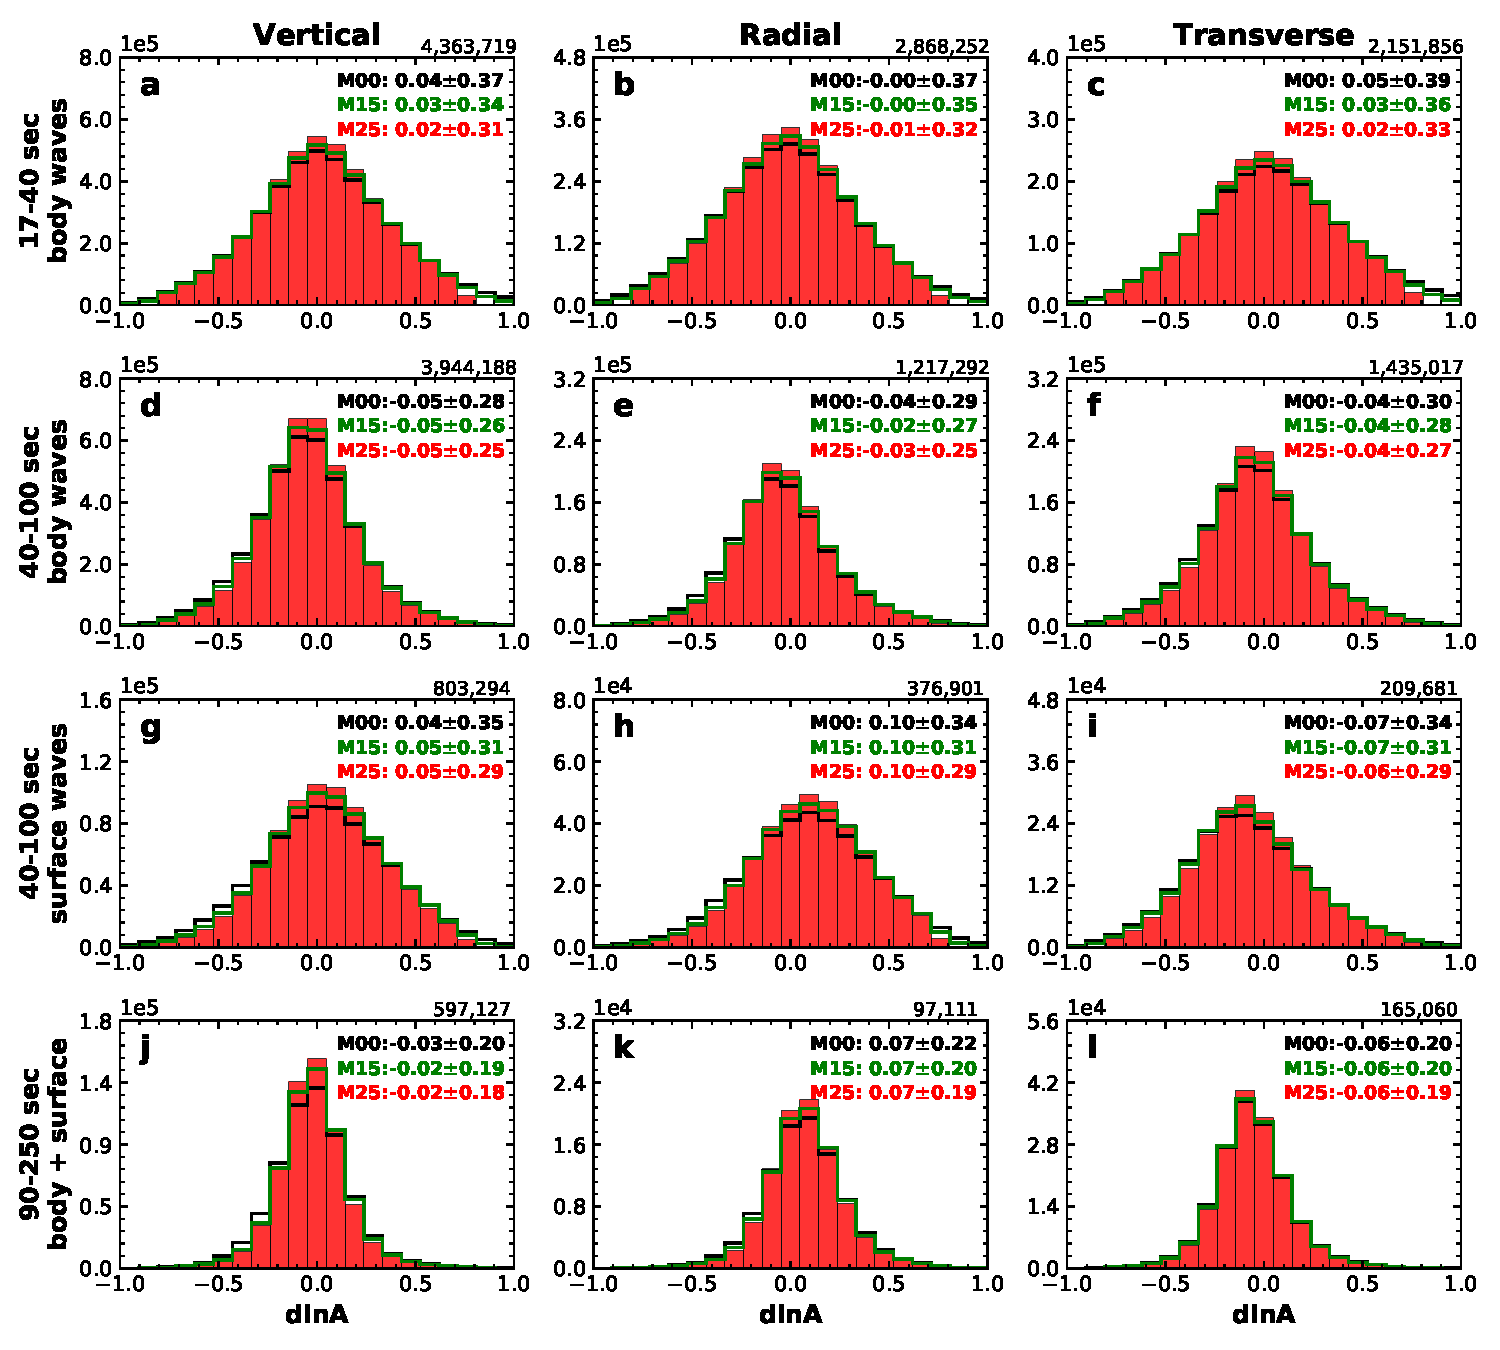
\includegraphics[width=\textwidth]{figures/dlna_histogram.pdf}
  \caption{Same as Fig.~\ref{fig:phase_hist} except for amplitude measurements. These measurements are currently not used in the inversion.}
  \label{fig:amp_hist}
\end{figure}

{\color{red} Wenjie: Also include the P arrival measurements here.}

\section{Model evaluation}

In this section we evaluate model GLAD-M25 further based on a point-spread function resolution analysis as well as a ``held-out'' dataset, that is, a set of data not used in the actual structural inversion.

\subsection{Point-spread function analysis}

Checkboard tests or tests involving a chosen known structure, e.g., a plume or slab,
are frequently used to evaluate resolution in a tomographic inversion.
Such tests are extremely expensive in FWI and adjoint tomography, because they require roughly the same computational resources as the actual inversion.
In lieu of such tests,
we performed two point-spread function analyses~\citep{fichtner2011resolution,zhu2015seismic,bozdaug2016global}.

\subsection{Held-out dataset}

Following the approach of \cite{tape2009adjoint}, \cite{chen2015multiparameter}, and \cite{bozdaug2016global},
we selected 360 earthquakes that were not used in the actual inversion.
This held-out dataset consists of all magnitude 6.3--7.0 earthquakes in the global CMT catalog that were not used in the inversion.
We chose larger events to generate as many measurements as possible.
We calibrated the centroid time and scalar moment using a grid search based on 3D synthetics calculated in GLAD-M25.
Fig.~\ref{fig:events_360} summarizes the properties of the held-out database.

\begin{figure}
  \centering
  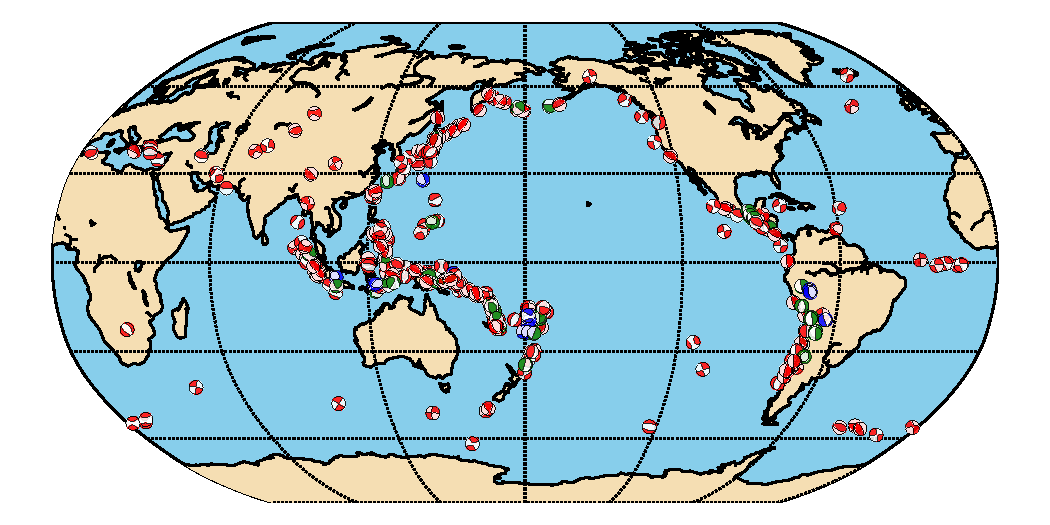
\includegraphics[width=\textwidth]{figures/events_360.pdf}
  \caption{Summary of the held-out database containing 360 earthquakes. Theses events were not used in the structural inversion. (a) Distribution of events, color coded by depth range as in Fig.~\ref{fig:event_1480}. (b) \& (c) Histograms of moment magnitude and depth.}
  \label{fig:events_360}
\end{figure}

First, we repeated the misfit assessment discussed in Section~\ref{section:Misfit assessment} for the held-out database.
Table~\ref{table:misfit_reduction_M15_M25_360} summarizes the reductions in misfit for the held-out database for model GLAD-M25 compared to GLAD-M15 as well a S362ANI combined with CRUST2.0.
It is comforting to see that the reductions are comparable to the
values tabulated in Table~\ref{table:misfit_reduction_M15_M25} for the actual inversion.
Overall, the reductions are slightly smaller, partly due to the fact that we did not conduct full CMT inversions for the held-out database.

\begin{table}[!htb]
  \centering
  %\label{tab:category}
  \begin{tabular}{|c|c|c|c|}
  \hline
  ~          &  Vertical (\%) & Radial (\%) &  Transverse (\%) \\
  \hline
  17--40~s                &          11.8 (29.2) &       14.1 (33.7) &       21.5 (43.4) \\
  40--100~s body waves    &          14.5 (26.2) &       12.9 (32.2)  &       16.9 (39.0) \\
  40--100~s surface waves &          29.3 (49.1) &       28.1 (49.4) &       23.7 (51.2) \\
  90--250~s               &          10.9 (30.9) &       14.3 (34.8)  &       24.0 (34.9) \\
  \hline
  \end{tabular}\\
  \caption{Changes in fit for 360 earthquakes not used in the inversion in the twelve measurement categories
between the new model, GLAD-M25, and its starting model, GLAD-M15, and, in parentheses, between GLAD-M25 and model S362ANI combined with CRUST2.0, which was the starting model for the GLAD-M15 inversion.}
  \label{table:misfit_reduction_M15_M25_360}
\end{table}

% \begin{table}[!htb]
%   \centering
%   %\label{tag:misfit_reduction_M00_M25_360}
%   \begin{tabular}{|c|c|c|c|}
%     \hline
%     ~          &  Vertical(\%) & Radial(\%) &  Transverse(\%) \\
%     \hline
%     17--40s                &         29.2 &       33.7 &       43.4 \\
%     40--100s body waves    &         26.2 &       32.2 &       39.0 \\
%     40--100s surface waves &         49.1 &       49.4 &       51.2 \\
%     90--250s               &         30.9 &       34.8 &       34.9 \\
%     \hline
%   \end{tabular}\\
%   \caption{Misfit Reduction from M00 to M25 for 360 earthquakes as held-out dataset}
%   \label{table:misfit_reduction_M00_M25_360}
% \end{table}

Second, we repeated the histogram comparisons discussed in Section~\ref{section:Histogram comparisons} for the held-out database.
We used a set of identical windows on all three components to assess
phase anomalies in models GLAD-M25, GLAD-M15, and S362ANI combined with CRUST2.0.
Fig.~\ref{fig:phase_hist_360} shows histograms of the resulting phase
measurements in all twelve measurement categories.
The total number of measurements exceeds 7.8~million.
As in the actual inversion,
we observe systematic decreases in all standard deviations in all twelve categories,
and we note a sharpening of the distributions centered around zero.

\begin{figure}
  \centering
  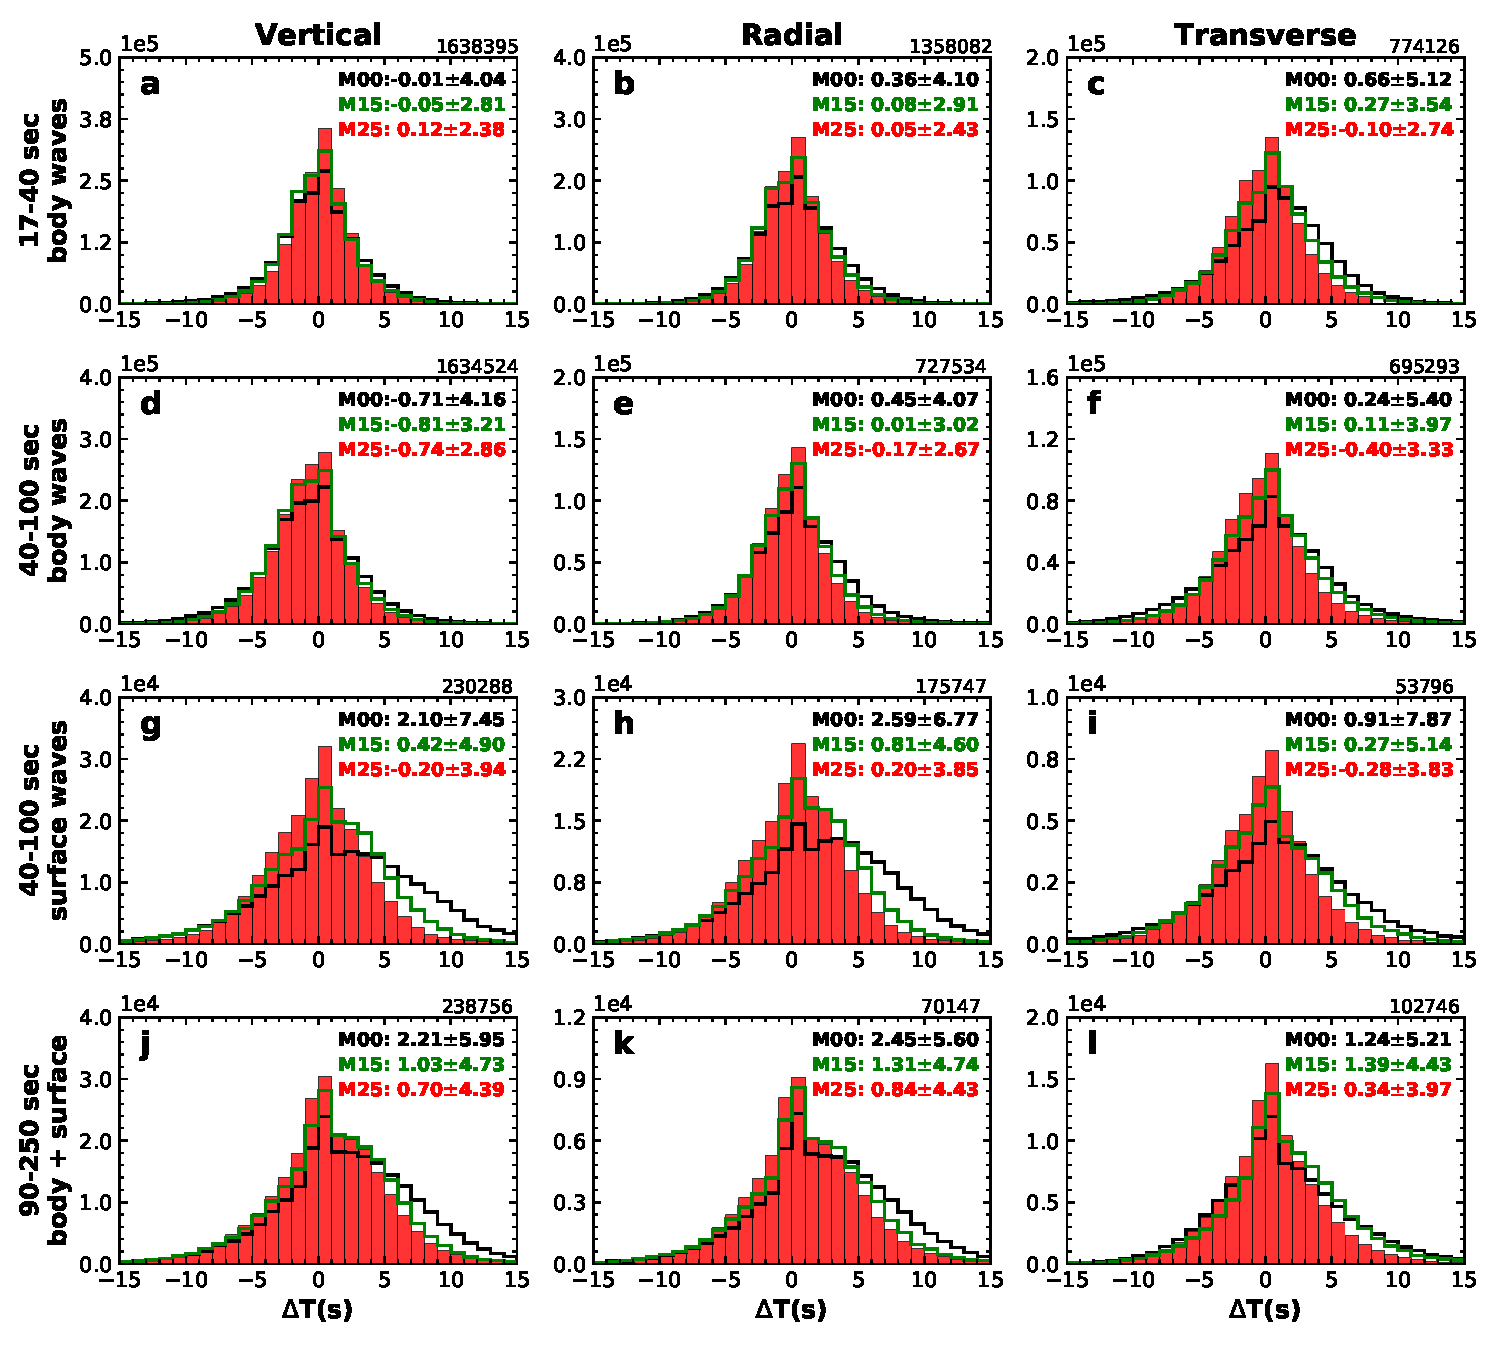
\includegraphics[width=\textwidth]{figures/dt_histogram_360.pdf}
  \caption{Histograms of phase measurements for the 360 events in the held-out database.}
  \label{fig:phase_hist_360}
\end{figure}

\section{Model GLAD-M25}

In this section we discuss model GLAD-M25 in some detail.
We begin with a global overview of the model before concentrating on specific geographical regions.
We conclude by highlighting various slabs and plumes in the model.

\subsection{Global structure}

We first examine model GLAD-M25 in the context of existing global tomographic models.
In Fig.~\ref{fig:global-vs} we compare global maps of the isotropic part of our shear wavespeed model with model S362ANI$+$M~\citep{moulik2014anisotropic},
which is an updated version of the starting model for the GLAD-M15 inversion,
and model S40RTS~\citep{ritsema2011s40rts}.
The range of perturbations in shear wavespeed varies from map to map, as indicated in the top left of each panel.
Overall, these models are in good agreement at the longest wavelengths, especially Glad-M25 and S362ANI$+$M.
The perturbations in GLAD-M15 tend to be larger than in the other models,
consistent with observations by~\cite{french2014whole},
whose model is also based on a form of waveform inversion.

\begin{figure}
  \centering
  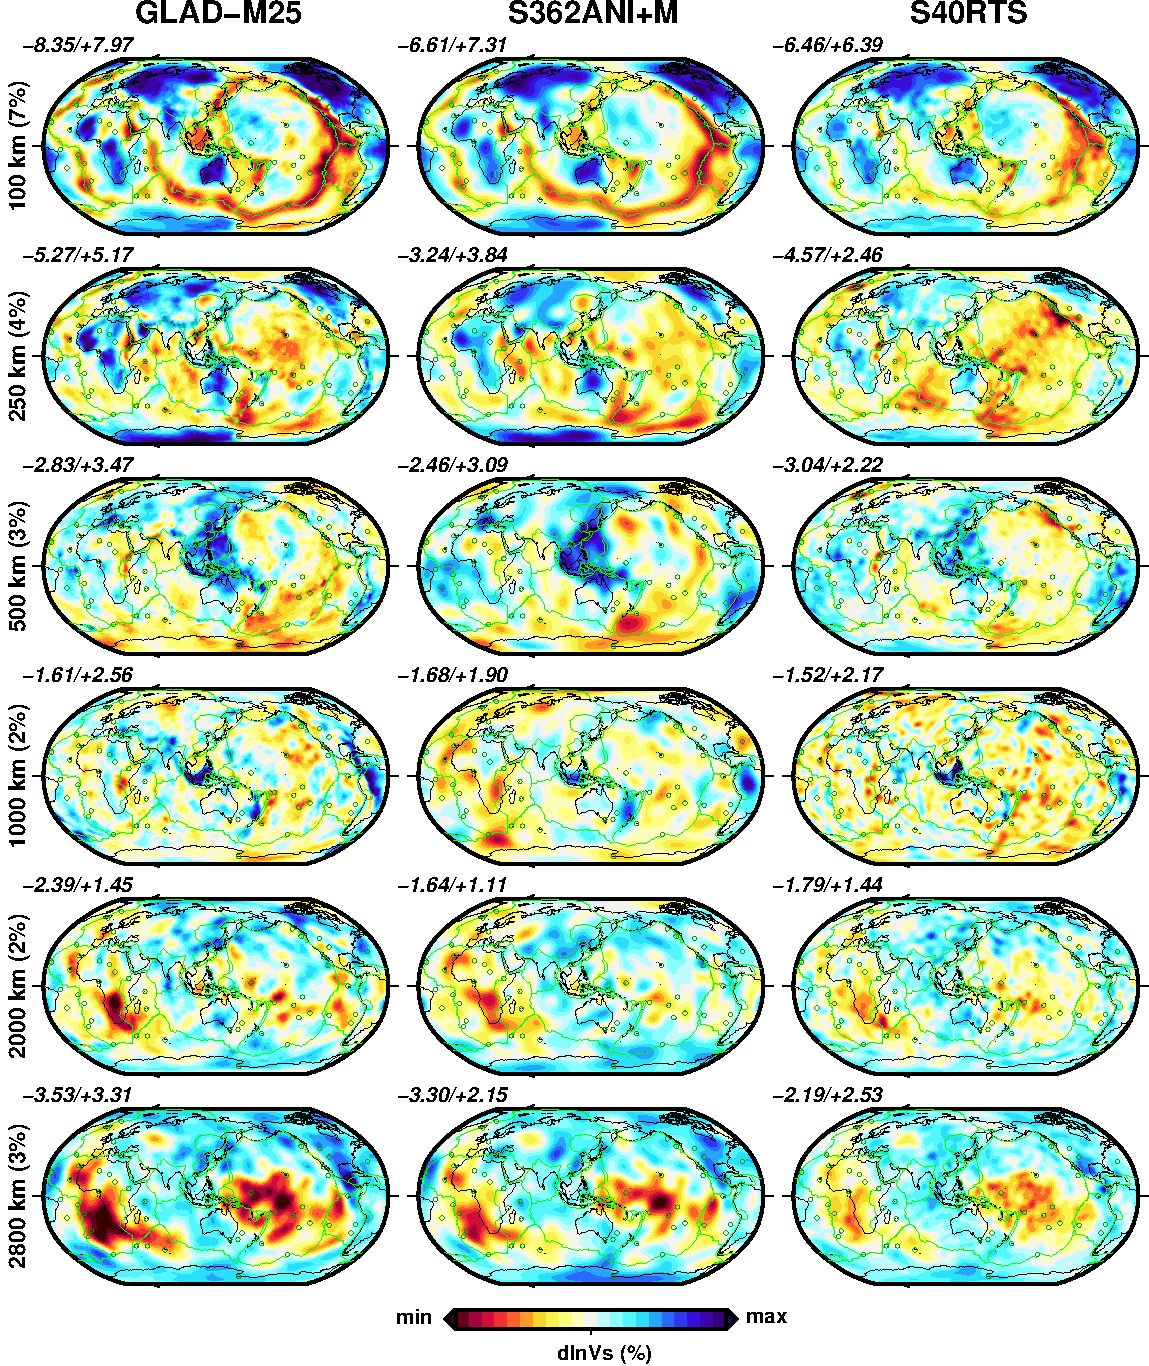
\includegraphics[width=0.9\textwidth]{figures/depth_slice/globe_vs.pdf}
  \caption{Map views of global shear wavespeed perturbations at various depths for  model
  GLAD-M25~(left column), S362ANI$+$M~\citep[middle column;][]{moulik2014anisotropic}
  and S40RTS~\citep[right column;][]{ritsema2011s40rts}.
  At a given radius,
  perturbations are calculated relative to each model's average.
  The range of perturbations in shear wavespeed varies from map to map, as indicated in the top left of each panel.
  The green circles denote locations of various
  hotspots~\citep{montelli2006catalogue}.
  The range of the colorbar is the same for each row,
  and its maximum value is indicated in parentheses on the left, after
  the depth.}
  \label{fig:global-vs}
\end{figure}

%\begin{figure}
%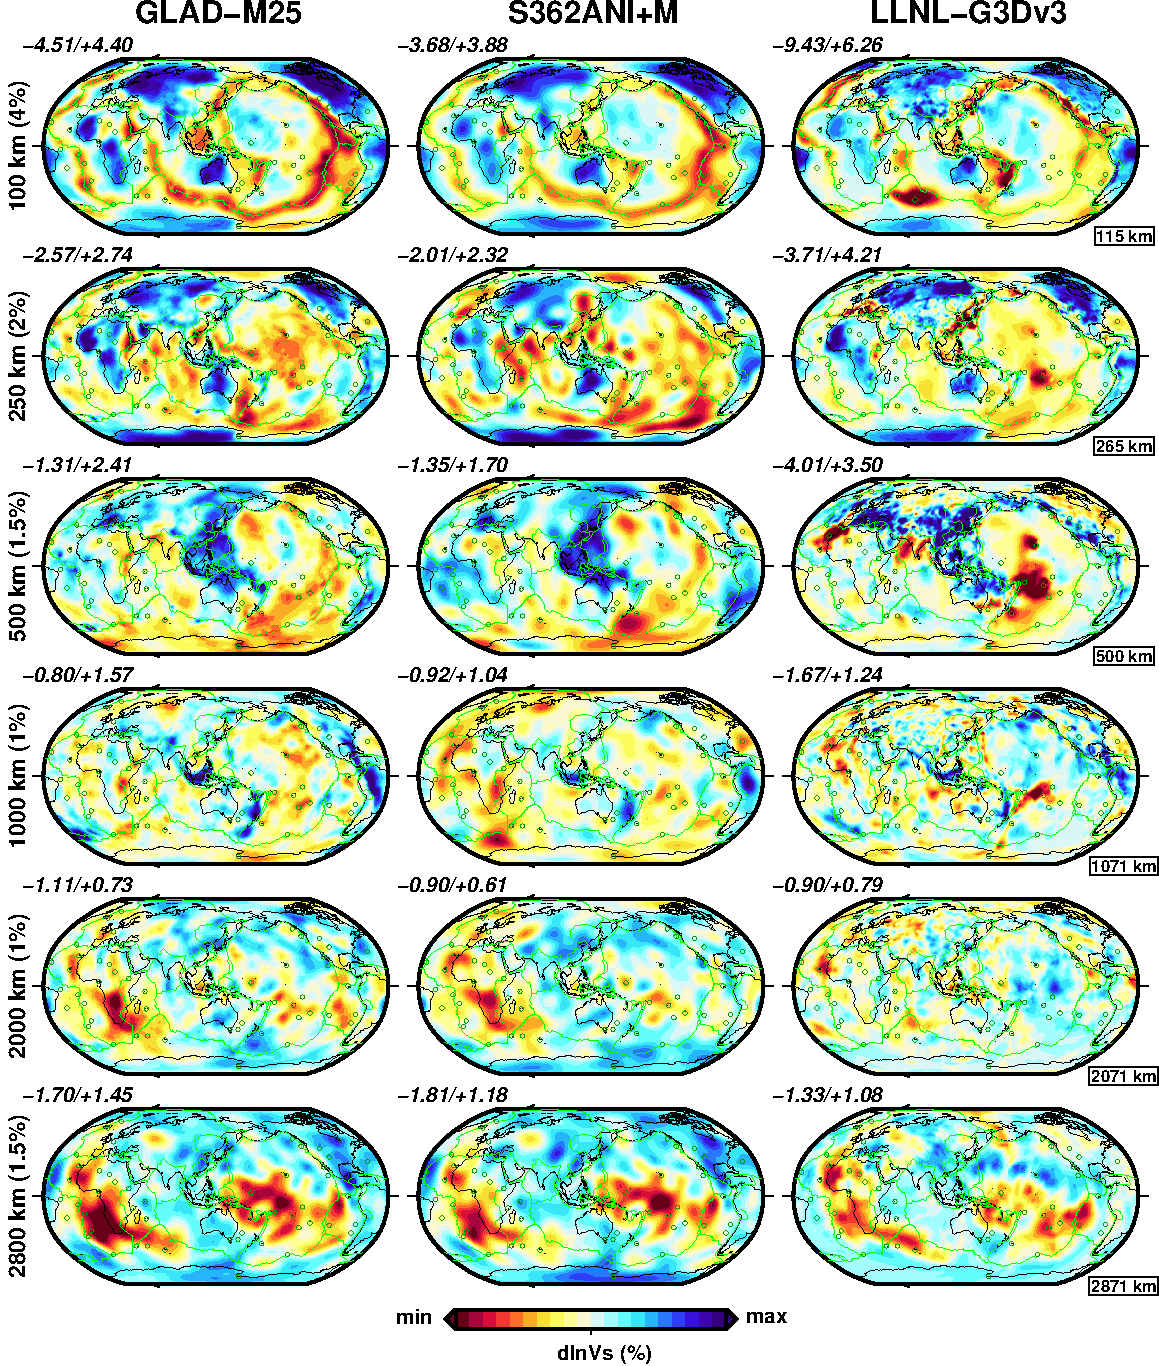
\includegraphics[width=0.9\textwidth]{figures/depth_slice/globe_vp_S362ANI-LLNL.pdf}
%  \caption{Map views of global $V_p$ variations at various depths for our model GLAD-M25(left column), S362ANI$+$M(middle column) and LLNL-G3Dv3(right column)\citep{simmons2012llnl}. For LLNL-G3Dv3, the depths is labeled on the right bottom based on its own mesh spacing. Other plotting conventions are used similar as in Figure \ref{fig:global-vs}.}
%\label{fig:global-vp}
%\centering
%\end{figure

An important aspect of our inversion is that it constrains shear and compressional waves simultaneously.
In Fig.~\ref{fig:global-vs} we compare global maps of our compressional wavespeed model with P models LLNL-G3Dv3~\citep{simmons2012llnl} and GAP-P4~\citep{fukao2013subducted}.
At a depth of 100~km,
GLAD-M25 shows prominent mid-oceanic ridges, cooling of the Pacific lithosphere, and the roots of numerous continental cratons.
In the upper mantle, LLNL-G3Dv3 exhibits the largest lateral variations,
e.g., very slow compressional wavespeeds at 500~km depth below Hawaii, Samoa, and Tahiti.
In the midmantle we can see remnants of subduction beneath South America, Indonesia,
and Tonga-Kermadec.
In the deep mantle, LLNL-G3Dv3 and GAP-P4 begin to fade out, but the long-wavelength patterns,
in particular the lowerparts of the Africa and Pacific superplumes, are very similar.

{\color{red} Wenjie: Note: add spherical harmonic analysis later.}

\begin{figure}
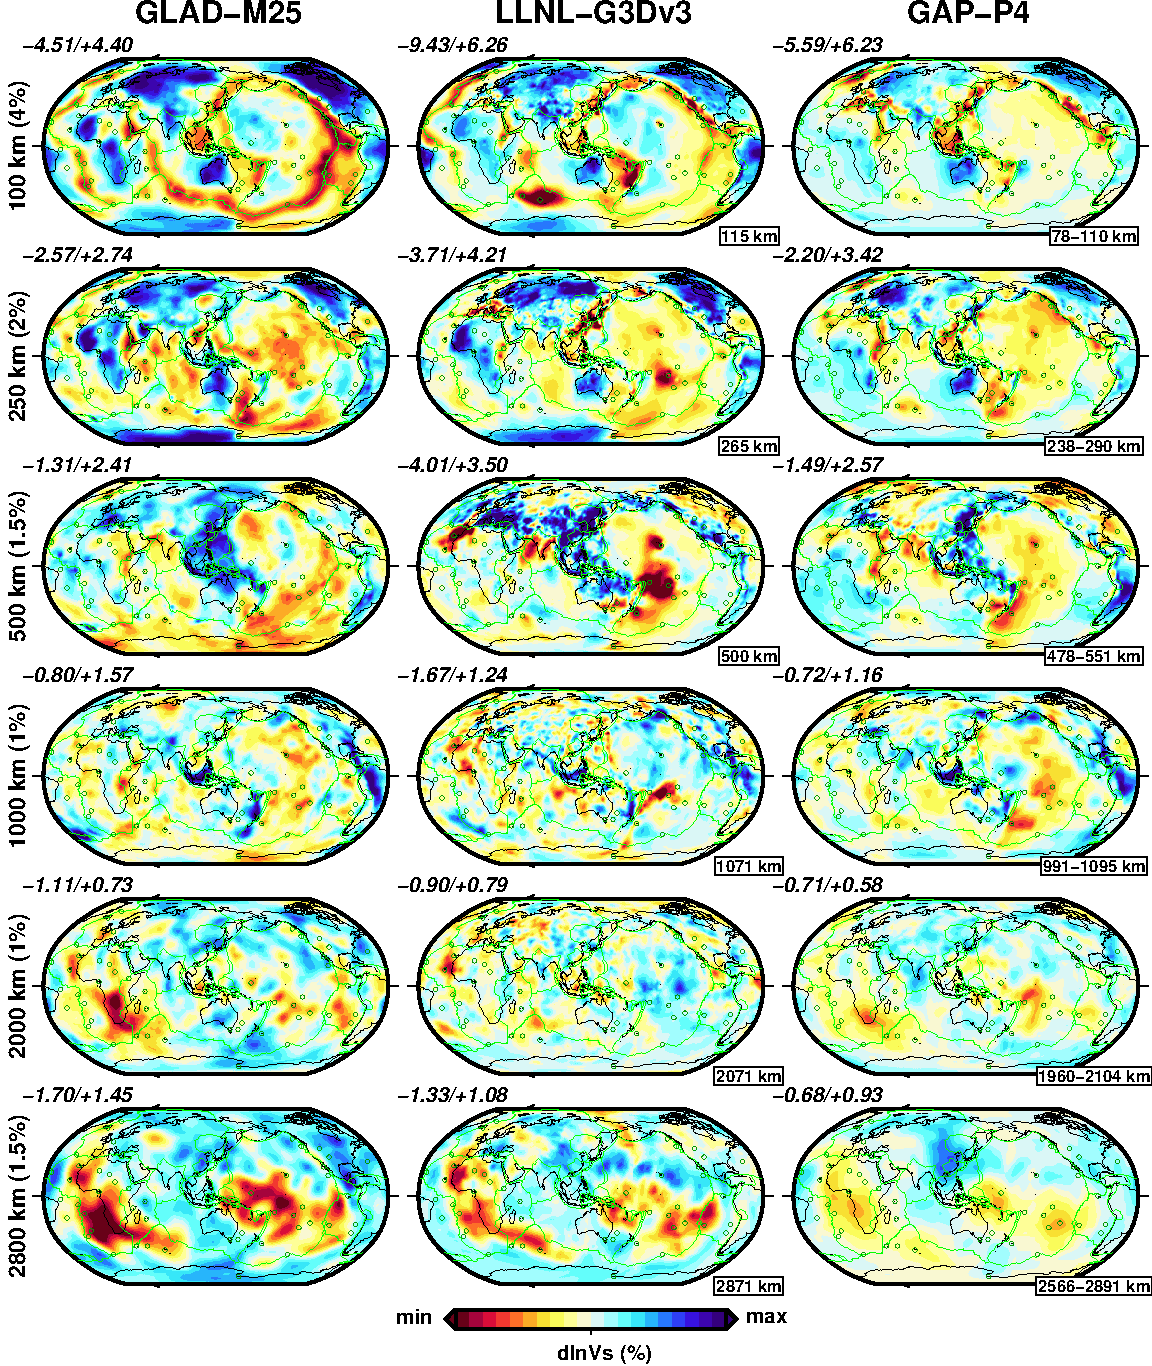
\includegraphics[width=0.9\textwidth]{figures/depth_slice/globe_vp_LLNL-GAP.pdf}
  \caption{Map views of global compressional wavespeed variations at various depths for model
  GLAD-M25 (left column), LLNL-G3Dv3 \citep[middle column;][]{simmons2012llnl} and
  GAP-P4~\citep[right column;][]{fukao2013subducted}.
  For LLNL-G3Dv3, depth ranges are labeled in the bottom right
  bottom of each panel. Other plotting conventions are as in Fig.~\ref{fig:global-vs}.}
\label{fig:global-vp}
\centering
\end{figure}

\subsubsection{North America}

\begin{figure}
\centering
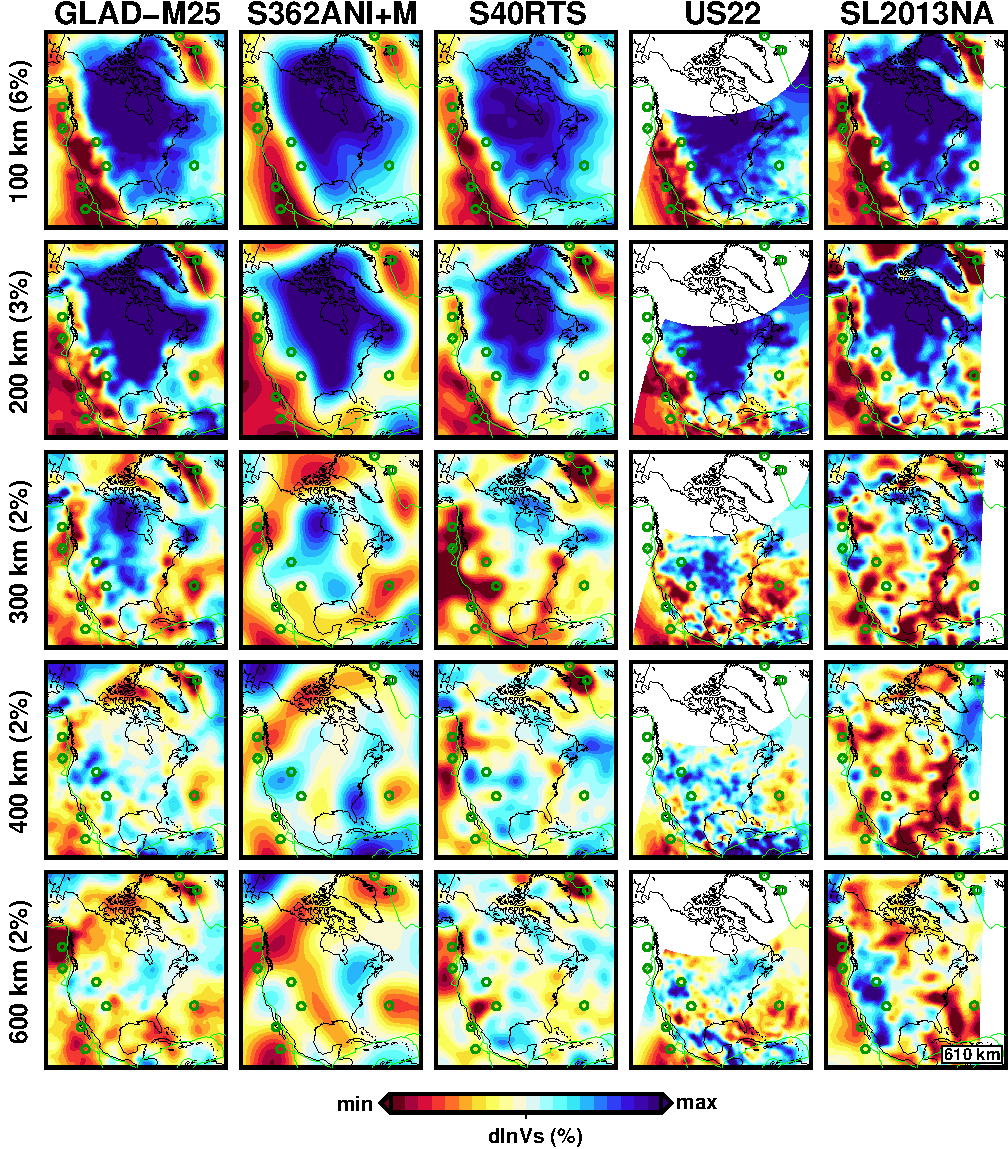
\includegraphics[width=0.9\textwidth]{figures/depth_slice/america_vs.pdf}
  \caption{Map views of isotropic shear wavespeed variations beneath North America 
  for model GLAD-M25 (first column) and several global (S362ANI$+$M and S40RTS)
  and regional~\citep[US22;][]{zhu2017radial} and~\citep[SL2013NA;][]{schaeffer2014imaging}
  models. Green circles denote the locations of hotspots. For SL2013NA, we
  show a depth of 610~km instead of 600~km, reflecting its model parametrization.}
\label{fig:america-vs}
\end{figure}

The deployment of USArray has dramatically increased data overage across the
continental United States.
In this section, we compare GLAD-M25 in this region with
with two global models, S362ANI$+$M and S40RTS, and two regional models,
US22~\citep{zhu2017radial} and SL2013NA~\citep{schaeffer2014imaging}.
US22 is a radially anisotropic model based on adjoint tomography using
USArray data from 180 regional earthquakes using 15--50~s
body waves and 25--150~s surface waves.
SL2013NA is a global upper-mantle shear wavespeed model based on multimode
surface waveform tomography primarily focused on North America.

North America is characterized by a large, high-wavespeed lithospheric craton,
bounded by the Rocky Mountain Front to the West and continental
margin to the East. On both sides the lithosphere has been deformed by
low wavespeed structures, thus forming sharp tectonic boundaries.

At a depth of 100~km, we observed that the edges of the craton are sharper in
GLAD-M15 than in the other two global models,
and quite similar in shape and sharpness to the two regional models.
We can clearly see impressions of the Snake River Plain (with Yellowstone)
and the Raton hotspot, which also have distinct slow expressions at depths of 200~km.
The core of the craton exhibits fast wavespeeds at depths reaching 300~km Northwest of
Hudson Bay.
In the regional models the craton has basically faded away at these depths.
The Wyoming and Medicine Hat Blocks show a very strong and thick lithospheric
root from shallow depths to $\sim$400~km, similar to US22 but
difficult to discern in SL2013NA.
Similar observations can be made for the Yavapai and
Mazatzal Blocks, which define the southern boundary of the large craton.

In the 200--400~km depth range, we observe a high wavespeed
anomaly within the Gulf of Mexico, which coincides spatially with the deepest
bathymetry and corresponds to a portion of ancient oceanic
Lithosphere~\citep{muller2008}.
A remnant of the Juan de Fuca plate,
with a high wavespeed footprint, is visible at depths of 300~km and 400~km,
where SL2013NA shows a much stronger anomaly.

In the North, we see a high wavespeed craton beneath Greenland which is partly
separated from the North American craton by low wavespeed structures beneath
Baffin Bay and the Labrador Sea, where the North American craton nicely follows
the coastline.
In the Northeast corner of the maps we see that the Iceland hotspot is very
prominent in GLAD-M25 in all depth ranges, similar to S40RTS but largely missing
in S362ANI$+$M. In the Northwest we see a clear imprint of the Aleutian
subduction zone in the 200--400~km depth range, comparable to SL2013NA but absent
in the other global models.

In the East, at 100~km depth,
we see ageing of the Atlantic lithosphere, comparable to the other global models
~\citep{muller2008, schaeffer2014imaging}.
All models show fast anomalies beneath Newfoundland and Nova Scotia extending to
depths of 300~km. The Bermuda hotspot shows a very nice slow wavespeed impression,
getting sharper and stronger at depths of 200~km and 300~km (note differences in
the scales of the maps).
The Caribbean slab, a relatively young subduction zone, is clearly
visible in our model in the 200--400~km depth range.
At greater depths,
GLAD-M25 shows a very distinct image of the Farallon slab,
but since it goes well beyond the depth range of this comparison,
we return to this feature in Section~\ref{section:slabs}.


\subsubsection{Europe}

Fig.~\ref{fig:europe-vs} shows isotropic shear wavespeed perturbations beneath Europe.
In addition to our model GLAD-M25, S362ANI+M and S40RTS, we included a regional
tomography model EU60\citep{zhu2015seismic} into our comparison. The EU60 uses
adjoint methods to iteratively inverse the crust and upper mantle structure
beneath the European continent and North Atlantic Ocean, by assimilating
190 earthquakes and 745 seismic station.

Europe is featured by the Trans-European Suture Zone(TESZ), separating the
Precambrian East European Craton(EEC) in the northeast and the Phanerozoic
Europe in the southwest.  The TESZ is very consistent across all the models,
even though is much sharper in GLAD-M25 and EU60.

In the north, we observed the high velocity anomaly beneath Central Graben in the
North Sea, and clearly separated from the EEC bounded at the western north, which is
explained as the lithospheric drip with delamination, as explained in
\cite{zhu2015seismic}.

In the south at the Mediterranean region, the tectonic settings is complex with the
existence of several regional plates. In the west of Mediterranean ocean, there is
Appennines-Maghrebides subductions, with the subduction retreat direction from South
(older, >30Ma)to North(younger, present), with its western border of back-arc basin
following along the coastline of East Spain and South France
\citep{Giordano2017Magmatic}. In our model, this is shown as fast velocity starting
from 400km and extend all the way to the mantle transition zones at 600km beneath the
Mediterranean Ocean, nicely following its west and east boundaries. At shallower depth
such as 100km, we observe low velocity structures, which is explained as the
back-arc extension associated with the roll-back. Compared to S362ANI+M and S40RTS,
our model shows much sharper features for the tectonic structures mentioned above.

Moving further to the east, at about 400km, there is clear fast anomaly lie
beneath the Dinarides Mountains, separating the Adria plate and Pannonian Basin,
indicating the subduction of Adria plate into the Euroasian plate.
This anomaly get sharper at 600km. The southern
part of it interacts with the Hellenic Arc subductions, which penetrate the mantle
transition zones and extend below 1,000 km in our model. We will discuss the Hellenic
Arc in details in the later sections. The Pannonian Basin is featured by low velocity
anomaly at the depth from 100 to 250km, then gradually transferred to high velocity
due to the subduction of Adria plate. The Anatolia plate is shown as slow velocity
anomaly in our model, sharpened from two other global models.

In the Central Europe, there is Cenozoic Ridge System, featured by the low velocity
anomaly, starting from Massif Central and extending to Eifel. Both the EU60 and
GLAD-M25 found slow anomaly lying beneath the northern par of Rhine Graben, explained
as the reservoir that fuels the Eifel hotspot, from 100km to 250km.

In the north of Atlantic Ocean, our model strengthened the slow anomaly near the
Atlantic Ocean Ridge, especially at the Iceland and Azores. The Iceland, becomes
much strong in our model in the upper mantle from 250km to 400km, compared to
S362ANI+M, extending all the way to the mantle-transition zone. On the other hand,
Azores, is a much shallower hotspot, with the slow anomaly extend at about 250km.

\begin{figure}
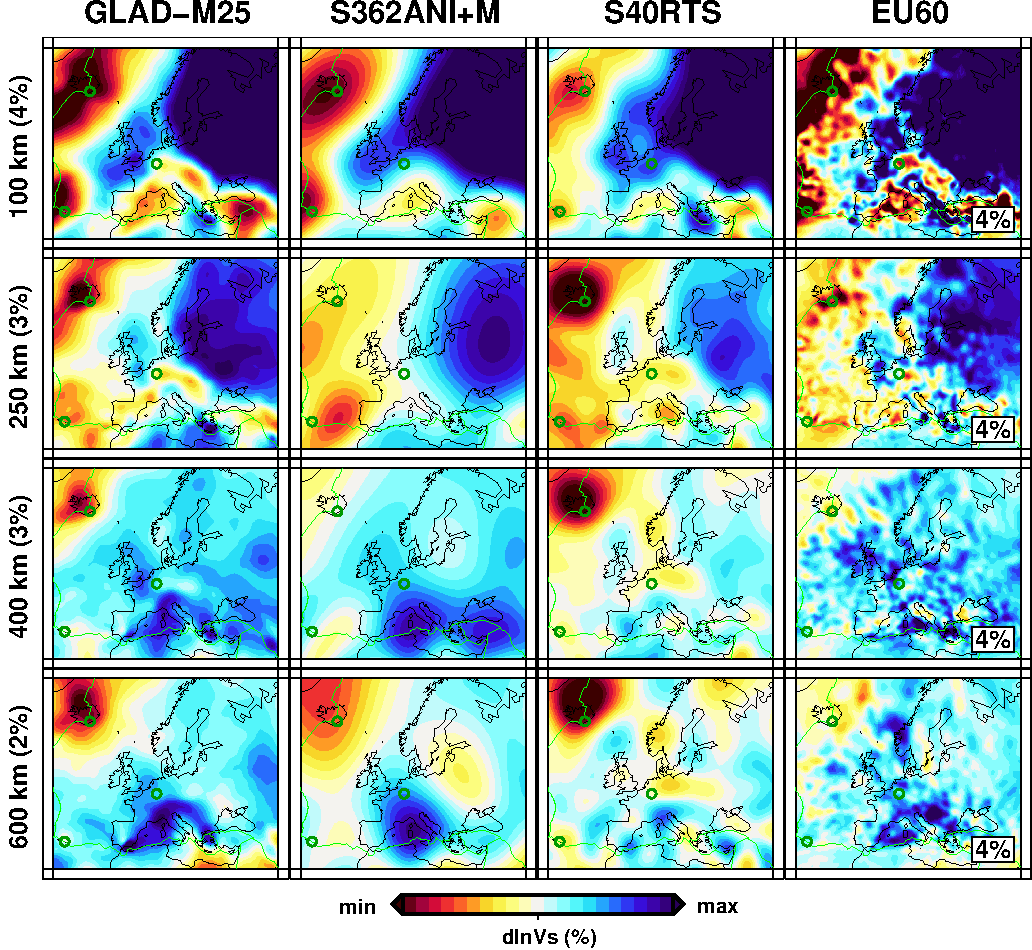
\includegraphics[width=0.9\textwidth]{figures/depth_slice/europe_vs.pdf}
  \caption{Map views of isotropic shear wavespeed variations beneath Europe for   
  model GLAD-M25 (first column), two global model (S362ANI$+$M and S40RTS), and
  one regional model~\citep[EU60;][]{zhu2015seismic}. For EU60, the range of the color
  bar is 4\% at all depths, as indicated in the bottom right bottom of the panels.}
\label{fig:europe-vs}
\centering
\end{figure}

\subsubsection{Asia}

Asia, like Europe, has a complicated tectonic history, involving
interactions among the Indian, Eurasian, Australian, Pacific, and Philippine
plates.
Map views of GLAD-M15 centered on Asia are plotted in Fig.~\ref{fig:asia-vs},
together with S362ANI$+$M, S40RTS, and regional model EARA2014~\citep{chen2015multiparameter}.
EARA2014 is a transversely isotropic model based on adjoint
tomography, assimilating 1.7~million frequency-dependent traveltime
measurements from 227 earthquakes recorded by 1,869 seismic stations.
It has superior data coverage, mainly by incorporating data from the China Array.

The Southwestern part of China is dominated by the Himalayas,
expressing the collision between India and Eurasia.
GLAD-M25 exhibits strong high wavespeed anomalies in this area,
which extend all the way from 100~km to 600~km, narrowing and sharpening with depth,
in good agreement with EARA2014.
The Tibetan plateau shows relatively low wavespeeds
compared to its surroundings, including the Himalayas to its South and
the Tianshan Mountains to its North, consistent with the other global
and regional studies.

The southern part of Asia shows major tectonic activity between the
Philippine, Eurasian, and Australia plates.
The Sunda trench is visible as a distinct high wavespeed anomaly below 200~km,
nicely following the plate boundary.
This feature remains very sharp at 600~km and extends
down to 1000~km.
We discuss this subducting slab further in Section~\ref{section:slabs}.
The Manila and Philippine trenches are also much sharper in our model between 200~km and
600~km than in the other global models, and comparable to EARA2014.
The eastern edge of the map features a series of trenches following plate boundaries,
including Japan, Izu-Bonin, and Mariana.
These slabs are absent in the other global model,
but feature more prominently in EARA2014.
Along the northern edge we see low wavespeeds associated with the
Altai-Sayan and Baikal rift systems.
In terms of intra-plate activities,
at shallow depths we see clear low wavespeed impressions of the Hainan and Changbai volcanoes,
suggesting a lithospheric rather than deeper mantle origin.
The Sichuan basin, a very localized high-wavespeed structure, extends below
250~km depth. At 600~km, most models shows a large region of high wavespeed
beneath the Philippine plate, indicating ponding of ancient subducted plates.

\begin{figure}
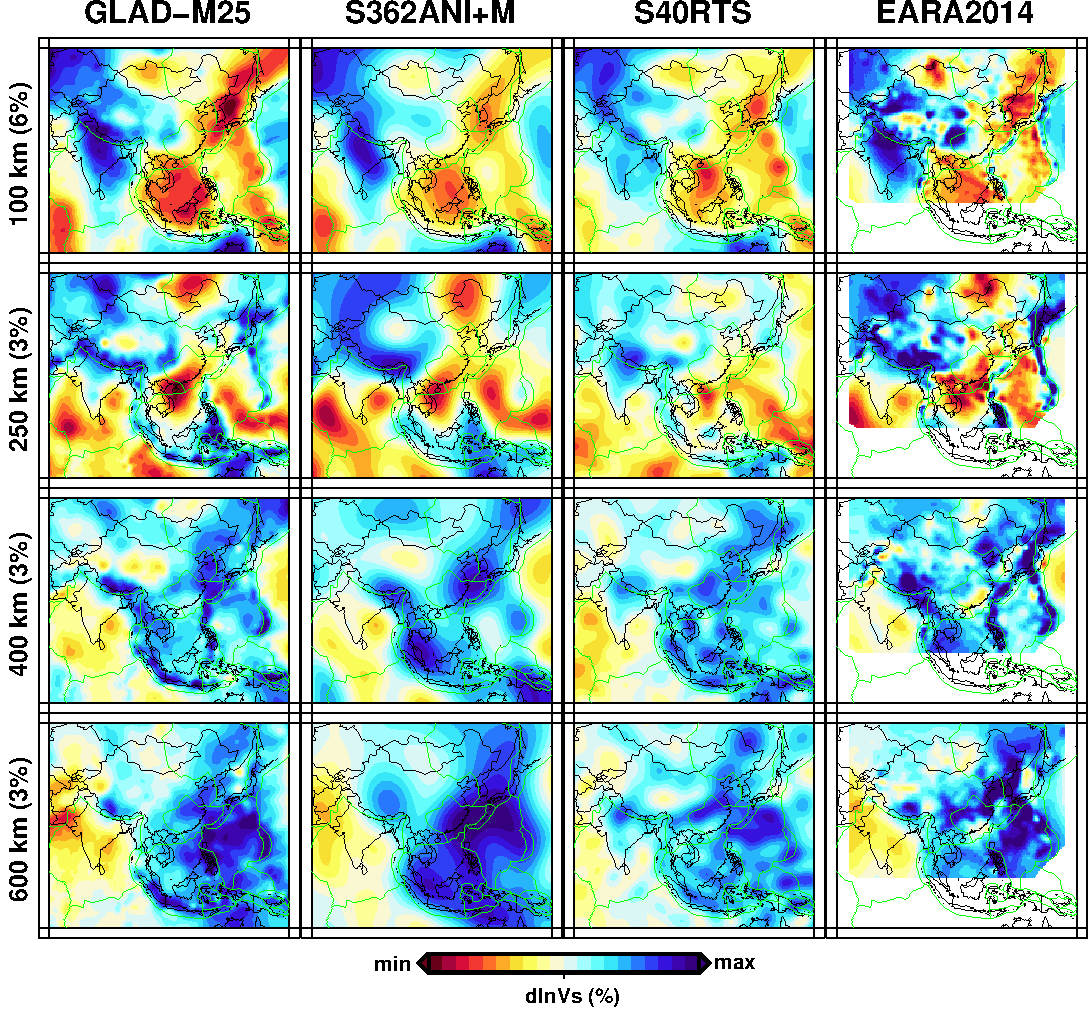
\includegraphics[width=0.9\textwidth]{figures/depth_slice/asia_vs.pdf}
  \caption{Map views of shear wavespeed variations beneath Asia for GLAD-M25~(first column),
  global models S362ANI$+$M (second column) and S40RTS (third column), and regional model EARA2014~\citep[last column;][]{chen2015multiparameter}.}
\label{fig:asia-vs}
\centering
\end{figure}

\subsubsection{South America}

\begin{figure}
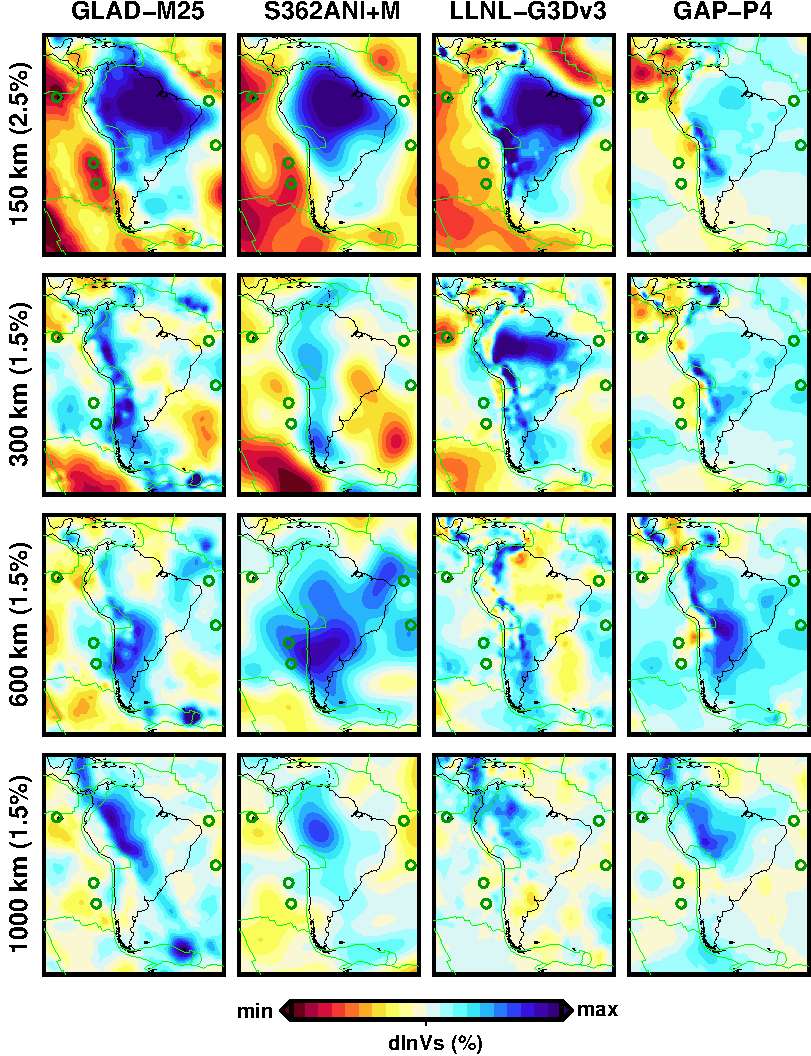
\includegraphics[width=0.9\textwidth]{figures/depth_slice/south_america_vp.pdf}
  \caption{Map views of compressional wavespeed variations beneath South America for GLAD-M25~(first column) and global models S362ANI$+$M, LLNL-G3Dv3~\citep{}, and GAP-P4~\citep{fukao2013subducted}.}
\label{fig:southamerica-vp}
\centering
\end{figure}

Fig.\ref{fig:southamerica-vp} shows the $V_p$ velocity in our model, together with 3
global models, S362ANI+M, LLNL-G3Dv3\citep{}, GAP-P4\citep{fukao2013subducted},
while the latter two are global $V_p$ models.

At 100km depth, the northern part of South America is covered by large area
of lithosphere craton, showing fast wave anomaly except GAP-P4. The fast anomaly
stays strong in LLNL-G3Dv3 while for GLAD-M25
and S362ANI+M it disappear at such depth.
At 300km, we are see a sharpened fast anomaly in the south subduction area
in GLAD-M25 compared to S372ANI+M. However, the shape and strength are very close
between GLAD-M25 and LLNL-G3Dv3 models. Moving to even larger depth, the features of
subductions becomes divergent between the north Peruvian slab and south Chilean slab.
At 600km, we observed a large chunk of fast anomaly in the Chilean slab,
indicating the slab is trapped and stagnant in the mantle transition zone. However,
the Peruvian slabs has penetrated the mantle transition zone and extend till 1000,
reaching the uppermost part of lower mantle, which is consistent with GAP-P4
\citep{fukao2013subducted}.

Besides, in the Pacific and Nazca plate, our models is sharpening the Galapagos,
San Felix and Juan Fernandez hotspot. In the Scotia plate, our models shows a very
strong expression of Scotia Arc subduction till 1000km, which is barely observable
in other models. In the Caribbean plate, we also observed fast anomaly, indicating
the Caribbean subduction.

\subsection{Plumes}
\label{section:plumes}

In this section, we will visit the plumes systems on the earth.

% %%%%%%%%%%%%%%%%%%%%%%%%%%%%%%%%%%%%%%%%%%%%%%%%%%%%%%%%
% Comment out for speed-up compile of latex file
% If not, the compilation will be slowed down quite a lot due
% to the insertion of PNG files.
% %%%%%%%%%%%%%%%%%%%%%%%%%%%%%%%%%%%%%%%%%%%%%%%%%%%%%%%%

%\begin{figure}[h]
%    \centering
%    \sidesubfloat[]{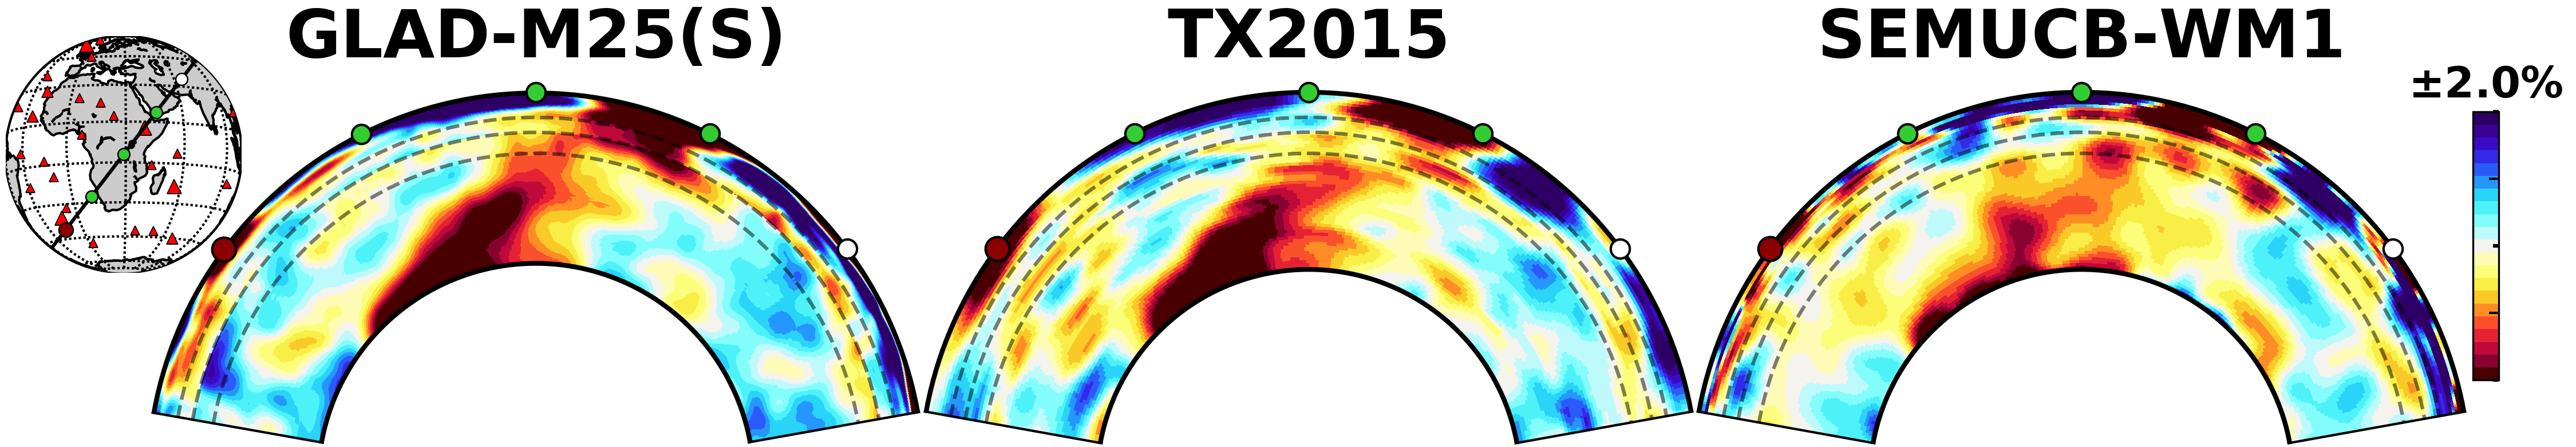
\includegraphics[width=0.98\textwidth]{figures/plumes/Afar.png}\label{fig:a}}\\[-1pt]
%    \sidesubfloat[]{
\includegraphics[width=0.98\textwidth]{figures/plumes/Bermuda_Canary.png}\label{fig:b}}\\[-1pt]
%    \sidesubfloat[]{
\includegraphics[width=0.98\textwidth]{figures/plumes/CapeVerde_Hoggar.png}\label{fig:c}}\\[-1pt]
%    \sidesubfloat[]{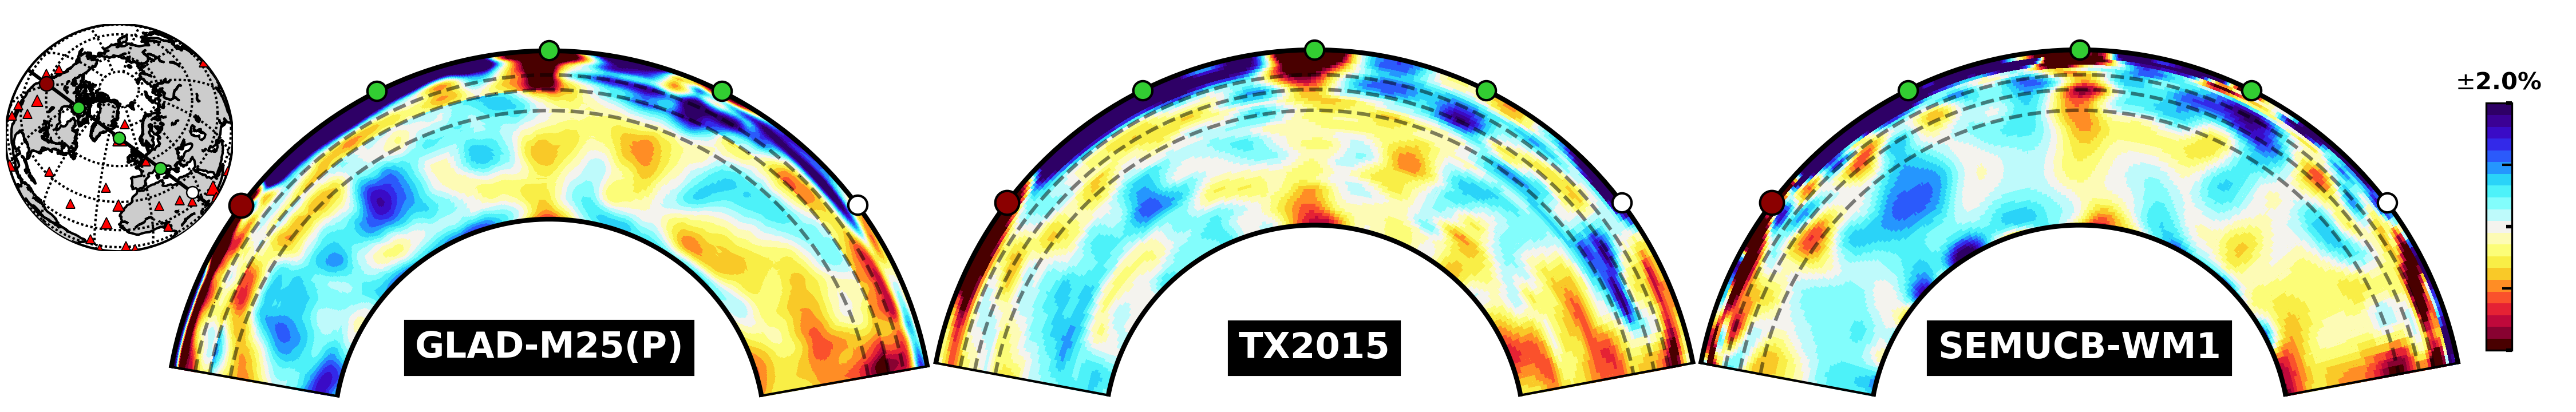
\includegraphics[width=0.98\textwidth]{figures/plumes/Iceland_Eifel.png}\label{fig:d}}\\[-1pt]
%    \sidesubfloat[]{
\includegraphics[width=0.98\textwidth]{figures/plumes/Canary_Iceland.png}\label{fig:e}}\\[-1pt]
%    \sidesubfloat[]{
\includegraphics[width=0.98\textwidth]{figures/plumes/Hoggar_AFAR.png}\label{fig:f}}\\[-1pt]
%    \sidesubfloat[]{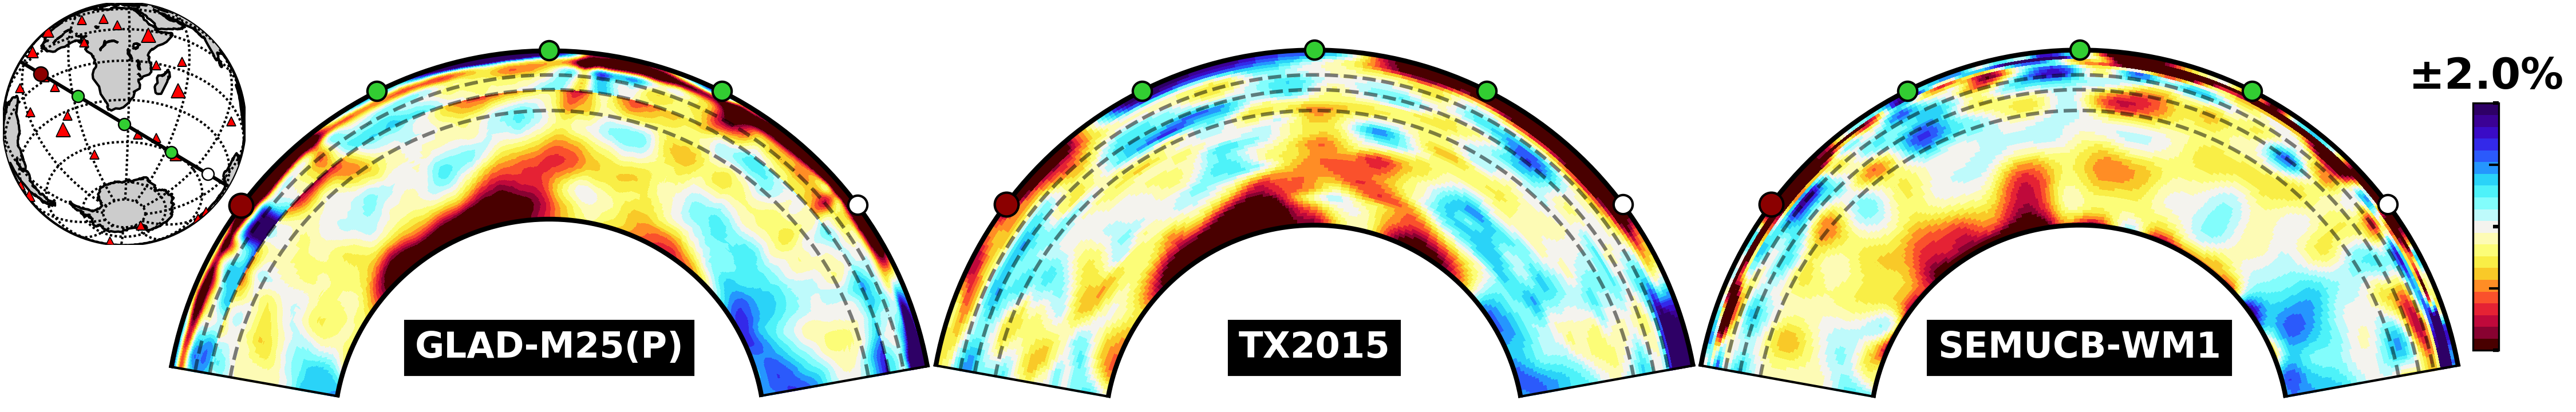
\includegraphics[width=0.98\textwidth]{figures/plumes/Marion3_Kerguelen.png}\label{fig:g}}\\
%    \caption{Vertical cross sections of perturbations of shear wave velocity Vs of plumes near the AFAR region.}
%\end{figure}

%\begin{figure}[h]
%    \centering
%    \sidesubfloat[]{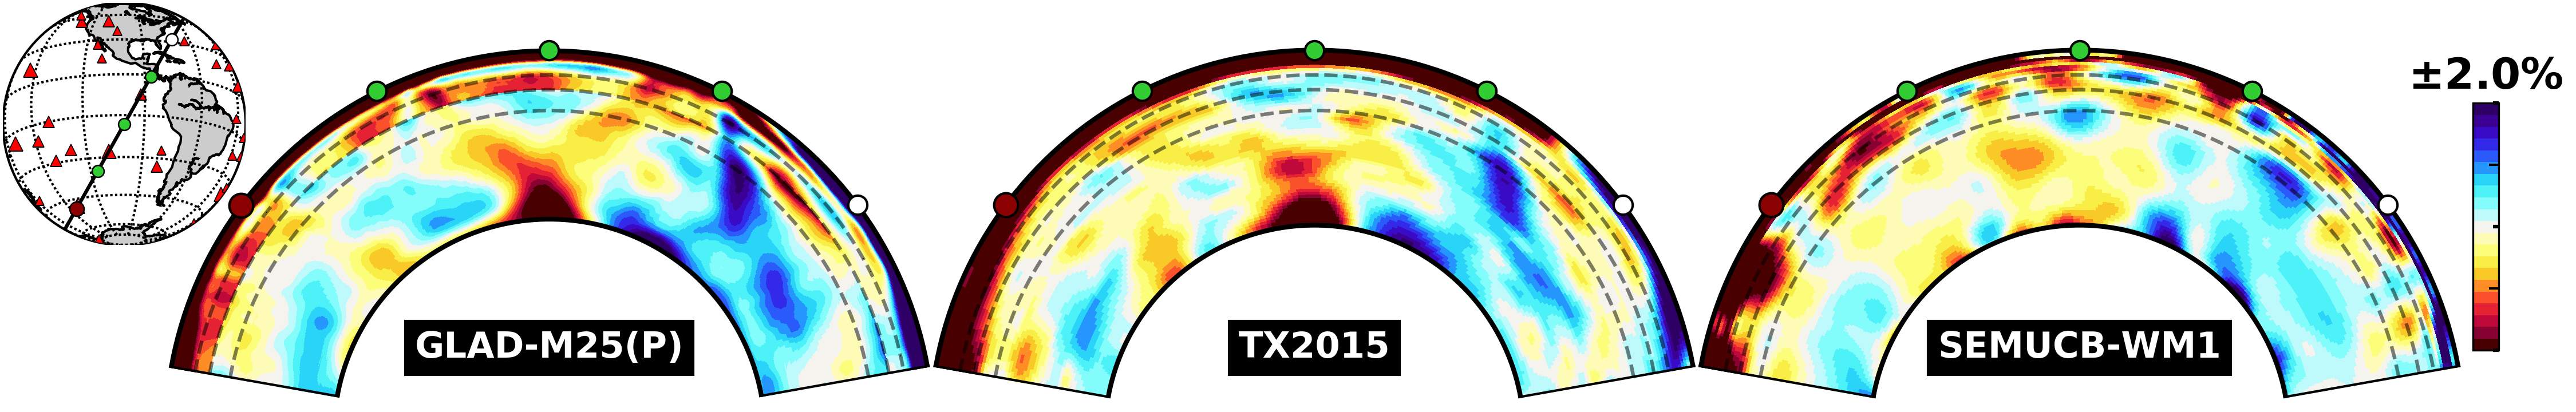
\includegraphics[width=0.98\textwidth]{figures/plumes/Easter_Galapagos.png}\label{fig:a}}\\[-1pt]
%    \sidesubfloat[]{
\includegraphics[width=1.0\textwidth]{figures/plumes/Macdonald_Yellowstone.png}\label{fig:b}}\\[-1pt]
%    \sidesubfloat[]{
\includegraphics[width=1.0\textwidth]{figures/plumes/Pitcairn_Guadalupe.png}\label{fig:c}}\\[-1pt]
%    \sidesubfloat[]{
\includegraphics[width=1.0\textwidth]{figures/plumes/Samoa_Hawaii.png}\label{fig:d}}\\[-1pt]
%    \sidesubfloat[]{
\includegraphics[width=1.0\textwidth]{figures/plumes/Samoa_MarquesasS1.png}\label{fig:e}}\\[-1pt]
%    \sidesubfloat[]{
\includegraphics[width=1.0\textwidth]{figures/plumes/Tahiti_Macdonald.png}\label{fig:f}}\\
%    \caption{Vertical cross sections of shear wave velocity perturbations of plumes in the pacific region.}
%\end{figure}

\subsection{Slabs}
\label{section:slabs}

In this sections, we will visit some of the well-known subduction zones.

\newpage


\section{Conclusion}

In summary,
the new model performs well for the held-out dataset, both in terms of misfit reductions and measurement distributions in all twelve measurement categories.
We expect to see similar behavior for any future earthquakes.


Seismology is driven by data. Back into time, seismologists would look at
single seismograms and pick valuable information out the them. Now, we have
ten thousands of seismograms deployed globally and it will be a pity not
to take all the information we have. Even though GLAD-M25 is following-up
of GLAD-M15. It has many superior advantages and improvements. We increase
the dataset from 253 to 1480 earthquakes, with carefully inverted sources
in the 3D earth structures. We have 360 earthquakes used in the test
dataset, which is already larger than the most of the dataset other people used
for their inversion. We culled every seismograms from various data centers,
thanks to the open environment and data sharing spirit of our seismology community.
With very careful checks by assessing the integrity of instrument response
and deployment, evaluating the signal-to-noise ratios, picking the time windows
using over 20 criteria, cleaning windows by their statistical behavior, and
calculating weights to balance the uneven distribution of earthquakes and
seismic stations, we really have done a lot to ensure the cleanness of the
data assimilated into our inversion and make sure every piece of value information
will be used but rejecting the crap data.

There are also quite a lot of technique challenges on the way but we are seeking
the most cutting-edge technologies to solve them. ADIOS was introduced to save mesh
and kernel related data, since we are saving petabytes of wavefiled snapshots
in a few hours of simulation and it is critical even for the most advanced
supercomputers in the world. ASDF is developed by us to store the seismograms
since we have ten millions of time series data from thousands of earthquakes.
We have to get access and process them in a very efficient manner that most of
the existing data format just won't meet our requirements. To handle the complex
inversion workflow, we are working RADICAL group to develop the workflow management
tools that will help manage every piece of task and make the user aware if there
is anything bad happened during the computation. Those tools that help the
automation of the workflow, is the "guard" that stand there and monitor things
to make sure our scientific results away from contamination. Besides, the
developer of SPECFEM packages, they dedicate more than ten years of work,
to develop the software and make it fast, efficient and robust for global scale of simulation.
They are working closely with hardware vendors such as Cray, IBM and NVidia to adapt
the code to architecture of the most advanced supercomputers. We are soon
moving our simulation to Summit, the world No.1 supercomputer at the Oak Ridge
National Lab.

\begin{acknowledgments}

%We want to give thanks to the Oak Ridge National Lab, for providing
%  excellent support and computational resource that facilitate our research.
%  We want to thanks IRIS and ORFEUS for providing seismic datas used in this
%  study. We want to acknowledge Hejun Zhu, Min Chen, Carl Tape and Qinya Liu,
%  for providing usefull tools and great suggetions these years.
%  We want to thanks Ebru Bozdag, for providing GLAD-M15, data and software
%  she used in the first generation model.

This research used resources of the Oak Ridge Leadership Computing Facility, which is a DOE Office of Science User Facility supported under contract DE-AC05-00OR22725.
Additional computational resources were provided by the Princeton Institute for Computational Science \& Engineering (PICSciE).
We acknowledge IRIS ({\tt iris.edu}) and ORFEUS ({\tt orfeus-eu.org}) for providing the data used in this study.
{\color{red} Wenjie: Please add all relevant data centers.} We thank Ryan Modrak, Ridvan Orsvuran, Frederik Simons, and James Smith for fruitful discussions.
The open source spectral-element software package SPECFEM3D\_GLOBE and the seismic measurement software package FLEXWIN used for this article are freely available via the Computational Infrastructure for Geodynamics (CIG; {\tt geodynamics.org}). This research was supported by NSF grant~1644826.

\end{acknowledgments}

\newpage

\appendix

\section{Spherical harmonic model expansion}

{\color{red} Wenjie, to save space, this appendix could also go in the supplementary online material.} 

In this appendix we express model GLAD-M25 in a spherical harmonic basis
to facilitate easy plotting, analysis, and comparisons with other models.
The resulting spherical harmonic model should only be used for these purposes, not for numerical simulations, which should always be based on the fully 3D spectral-element mesh.

To accomplish the transformation,
we first need to transform our 3D mesh --- which includes ellipticity, topography \& bathymetry, and undulations on internal boundaries --- into a spherical volume.
After these adjustments, we obtain a spectral element mesh for a perfect sphere,
that is, the sort of mesh we use for spherically symmetric earth models, such as PREM~\citep{PREM}.

In the spherical mesh, the model may be expressed in the form
\begin{equation}
    m(\mathbf{x})=\sum_{\mathrm{elem}}\sum_{\alpha,\beta,\gamma}m^{\alpha\beta\gamma}\,h_{\alpha}(\xi)\,h_{\beta}(\eta)\,h_{\gamma}(\zeta)\,
    \quad ,
\end{equation}
where~$h_\alpha$ denotes a Lagrange polynomial, and where we have used the invertible mapping
\begin{equation}
    \mathbf{x}=\mathbf{x}(\xi,\eta,\zeta)
    \label{eq:map}
\end{equation}
between spatial points~$\mathbf{x}=\{x,y,z\}$ and Gauss-Lobatto-Legendre (GLL) points in the reference element~$\{\xi,\eta,\zeta\}$~\citep{KoTr99}.

Our goal is to expand our spectral-element model in a spherical harmonic basis, i.e.,
\begin{equation}
    m(\mathbf{x})=\sum_{n=0}^N\sum_{\ell = 0}^L\sum_{m=-\ell}^\ell {}_nC_{\ell m}\,R_n(r)\,Y_{\ell m}(\theta,\phi)
    \quad ,
    \label{eq:m}
\end{equation}
where~$r$ denotes the radius, $\theta$ colatitude, and~$\phi$ longitude.
We choose a radial basis of the form~$R_n(r)$\,, $n=0,\ldots,N$\,,
e.g., layers or B-splines.
These radial basis functions need to be chosen sufficiently dense to mimic the density of the radial spectral element mesh.
The radial basis may or may not be orthogonal,
i.e.,
\begin{equation}
    \int_b^a R_{n'}(r)\,R_{n}(r)\,r^2\mathrm{d}r = A_{n'n}
    \quad ,
    \label{eq:R}
\end{equation}
where~$b$ denotes the radius of the CMB and~$a$ the free surface.
The matrix elements~$A_{n'n}$ define a positive definite matrix which is invertible.
As lateral basis functions we use fully normalized spherical harmonics~$Y_{\ell m}(\theta,\phi)$\,, $\ell=0,\ldots,L$ and $m=\mbox{}-\ell,\ldots,\ell$\,, i.e.,~\citep{DT98}
\begin{equation}
    \int_0^{2\pi}\int_0^\pi Y^*_{\ell'm'}(\theta,\phi)\,Y_{\ell m}(\theta,\phi)\,\sin\theta\,\mathrm{d}\theta\,\mathrm{d}\phi = \delta_{\ell' \ell}\,\delta_{m'm}
    \quad ,
    \label{eq:Y}
\end{equation}
where an asterisk denotes complex conjugation.
The maximum degree~$L$ needs to be chosen to resolve the spectral-element mesh laterally.

To obtain the expansion coefficients~${}_nC_{\ell m}$\,, we multiply Eqn.~(\ref{eq:m}) by
$R_{n'}(r)\,Y^*_{\ell' m'}(\theta,\phi)$ and integrate over the volume of the mantle and crust,~$V$\,, using Eqns.~(\ref{eq:R} and~(\ref{eq:Y}):
\begin{equation}
    \int_V m(\mathbf{x})\,R_{n'}(r)\,Y^*_{\ell' m'}(\theta,\phi)\,\mathrm{d}^3\mathrm{x}=\sum_{n=0}^N {}_nC_{\ell' m'}\,A_{n'n}
    \quad ,
\end{equation}
We evaluate the integral on the left using GLL quadrature~\citep{KoTr99}:
\begin{equation}
    \sum_{\mathrm{elem}}\sum_{\alpha,\beta,\gamma}\omega_\alpha\,\omega_\beta\,\omega_\gamma\,m^{\alpha\beta\gamma}\,J^{\alpha\beta\gamma}\,R_{n'}^{\alpha\beta\gamma}\,Y_{\ell'm'}^{*\,\alpha\beta\gamma}
    =\sum_{n=0}^N {}_nC_{\ell' m'}\,A_{n'n}
    \quad .
\end{equation}
Here~$\omega_\alpha$ denotes a GLL quadrature weight,
$J_{\alpha\beta\gamma}$ the Jacobian of the mapping~(\ref{eq:map}) evaluated on the GLL points,
and $R_{n'}^{\alpha\beta\gamma}$ and $Y_{\ell'm'}^{*\,\alpha\beta\gamma}$ the values of the radial and spherical harmonic basis functions at a GLL point.

Finally, the desired model coefficients may be obtained ---one combination of $n$\,, $\ell$\,, and $m$ at a time--- via
\begin{equation}
    {}_nC_{\ell m}=\sum_{n'}A^{-1}_{nn'}\sum_{\mathrm{elem}}\sum_{\alpha,\beta,\gamma}\omega_\alpha\,\omega_\beta\,\omega_\gamma\,m^{\alpha\beta\gamma}\,J^{\alpha\beta\gamma}\,R_{n'}^{\alpha\beta\gamma}\,Y_{\ell m}^{*\,\alpha\beta\gamma}
    \quad ,
    \label{eq:Cnlm}
\end{equation}
where~$A^{-1}$ denotes the inverse of the~$N\times N$ matrix~$A$.
Expressions of the form~(\ref{eq:Cnlm}) are commonplace in spectral-element simulations,
and thus easily calculated.
The power per degree~$\ell$ may be calculated via~\citep[][Eqn.~B.95]{DT98}
\begin{equation}
    \sigma_\ell^2=\frac{1}{2\ell+1}\,\sum_{n=0}^N\sum_{m=-\ell}^\ell|{}_nC_{\ell m}|^2
    \quad .
\end{equation}

Instead of the complex spherical harmonic model expansion~(\ref{eq:m}),
we may wish to use a real spherical harmonic expansion of the form~\citep[][Section~B.8, Eqn.~B.99]{DT98}
\begin{equation}
\begin{split}
    m(\mathbf{x}) \ = & \ \sum_{n=0}^N\sum_{\ell = 0}^L \left[ {}_na_{\ell 0}\,R_n(r)\,X_{\ell 0}(\theta)
   +\sqrt{2}\sum_{m=1}^\ell R_n(r)\,({}_na_{\ell m}\,\cos m\phi+{}_nb_{\ell m}\,\sin m\phi)\,X_{\ell m}(\theta)\right]
    \quad ,
\end{split}
    \label{eq:mreal}
\end{equation}
where~\citep[][Eqn.~B.30]{DT98}
\begin{equation}
    Y_{\ell m}(\theta,\phi)=X_{\ell m}(\theta)\exp(i m\phi)
    \quad ,
\end{equation}
and where
\begin{equation}
    {}_na_{\ell 0}=\sum_{n'}A^{-1}_{nn'}\sum_{\mathrm{elem}}\sum_{\alpha,\beta,\gamma}\omega_\alpha\,\omega_\beta\,\omega_\gamma\,m^{\alpha\beta\gamma}\,J^{\alpha\beta\gamma}\,R_{n'}^{\alpha\beta\gamma}\,X_{\ell m}^{\alpha\beta\gamma}
    \quad ,
\end{equation}
and for~$1\le m\le \ell$
\begin{equation}
    {}_na_{\ell m}=\sqrt{2}\,\sum_{n'}A^{-1}_{nn'}\sum_{\mathrm{elem}}\sum_{\alpha,\beta,\gamma}\omega_\alpha\,\omega_\beta\,\omega_\gamma\,m^{\alpha\beta\gamma}\,J^{\alpha\beta\gamma}\,R_{n'}^{\alpha\beta\gamma}\,X_{\ell m}^{\alpha\beta\gamma}\,(\cos m \phi)^{\alpha\beta\gamma}
    \quad ,
\end{equation}
\begin{equation}
    {}_nb_{\ell m}=\sqrt{2}\,\sum_{n'}A^{-1}_{nn'}\sum_{\mathrm{elem}}\sum_{\alpha,\beta,\gamma}\omega_\alpha\,\omega_\beta\,\omega_\gamma\,m^{\alpha\beta\gamma}\,J^{\alpha\beta\gamma}\,R_{n'}^{\alpha\beta\gamma}\,X_{\ell m}^{\alpha\beta\gamma}\,(\sin m \phi)^{\alpha\beta\gamma}
    \quad .
\end{equation}
The power per degree~$\ell$ may then be calculated via~\citep[][Eqn.~B.104]{DT98}
\begin{equation}
    \sigma_\ell^2=\frac{1}{2\ell+1}\,\sum_{n=0}^N\left[{}_na_{\ell 0}^2+\sum_{m=1}^\ell({}_na_{\ell m}^2+{}_nb_{\ell m}^2)\right]
    \quad .
\end{equation}

\newpage

\bibliographystyle{gji}
\bibliography{ref.bib}

\end{document}
